\section{Ground Control Station Setup}
\label{sec:GCS}
Now, in this section we first set up the Ground Control Station (GCS) as seen above in figure \ref{fig:GCS}. This section goes over the installation of VICON SDK, Pyvicon, MavProxy/Mavlink, and some corresponding package dependencies. This section is prone to some debugging against my best wishes, and everything is not really Plug N Play - Some resliences is required! 
\subsection{Hardware Required}
Please liaise with your corresponding supervisor/client and prepare a Linux running laptop with both Wifi and Ethernet Capability \footnote{Note that when runing Linux, some laptop's wifi card does not support Ubuntu 18.04, which you will need to rebuild the laptop to 20.04.} \footnote{Don't use Window Subsystem for Linux (WSL), it is a big hassle to figure out port communication permissions.} \footnote{Dual-booting your laptop into Linux/Window configuration is best if you only have a Window. \textbf{\textcolor{red}{Warnings however, dual-booting is intrinsicly an "easy to mess up" process with catastrophic consequences. Somes statistics for you, 2/12 students in my MSc cohort wiped out all their personal data while dual-booting their personal computer, so please backup all your data before dual-booting and make sure you know what you're doing!!!!}}}, a router (in the flight arena), and an ethernet cable (in the flight arena), as seen in figure \ref{fig:Hardware Requirement}.

\begin{figure}[H]
    \centering
    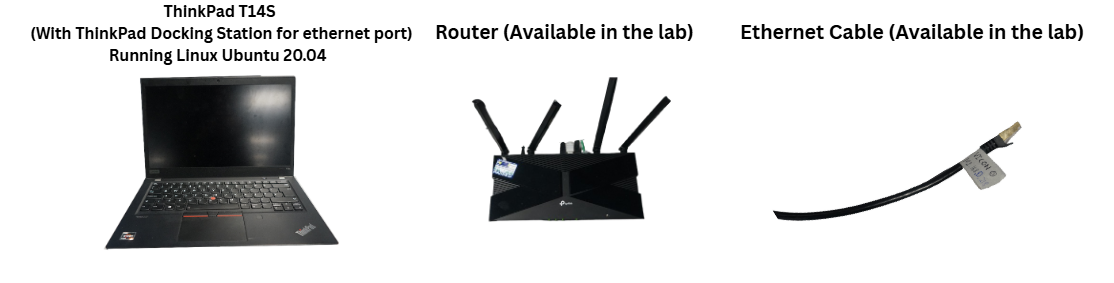
\includegraphics[width=1\linewidth]{Images/Hardware Requirements.png}
    \caption{Hardware Requirement}
    \label{fig:Hardware Requirement}
\end{figure}

\subsection{Setting Up Conda Virtual Environment}
Before we start setting up the softwares inside the virtual environment, let's set up a Virtual Environment (Venv). This step is to segregate your files you are going to install here away from the rest of the computer. This ensures that the package we download does not influence any other projects you have going on in your computer. (For example, you have 2 projects which requires 2 different version of a package, leading to a conflict). The use of venv is an industry pratice, so if you are starting out (Like me), make sure to use venv! To install the virtual environment, I use miniconda, a guide on installing can be found at \href{https://www.anaconda.com/docs/getting-started/miniconda/install/linux-install}{https://www.anaconda.com/docs/getting-started/miniconda/install/linux-install}

Once you have installed miniconda, Open a new virtual environment in python 3.10 named \textit{VICON} by typing:
\begin{lstlisting}
conda create -n VICON python=3.10
\end{lstlisting}

\begin{figure}[H]
    \centering
    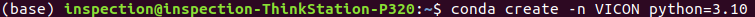
\includegraphics[width=1\linewidth]{Images/VirtualEnvironment/One.png}
    \caption{Setting up the virtual environment for Vicon.}
\end{figure}

When prompted, type \textit{y} to confirm the package installed. Once installed, activate the environment by pressing:

\begin{lstlisting}
conda activate VICON
\end{lstlisting}

It should look something like figure \ref{fig:VE2} below:

\begin{figure}[H]
    \centering
    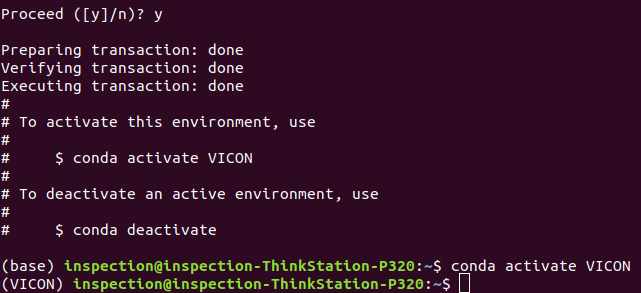
\includegraphics[width=1\linewidth]{Images/VirtualEnvironment/Two.png}
    \caption{Activating Virtual Environment}
    \label{fig:VE2}
\end{figure}

\subsection{Downloading VICON SDK}
Once we have set up the Conda environment, let's move on to downloading the VICON SDK now as aforementioned in section \ref{sec:TheBigPicture}. Visit \href{https://www.vicon.com/software/datastream-sdk/}{https://www.vicon.com/software/datastream-sdk/}, the website looks like figure \ref{fig:SDK1}: 
\begin{figure}[H]
    \centering
    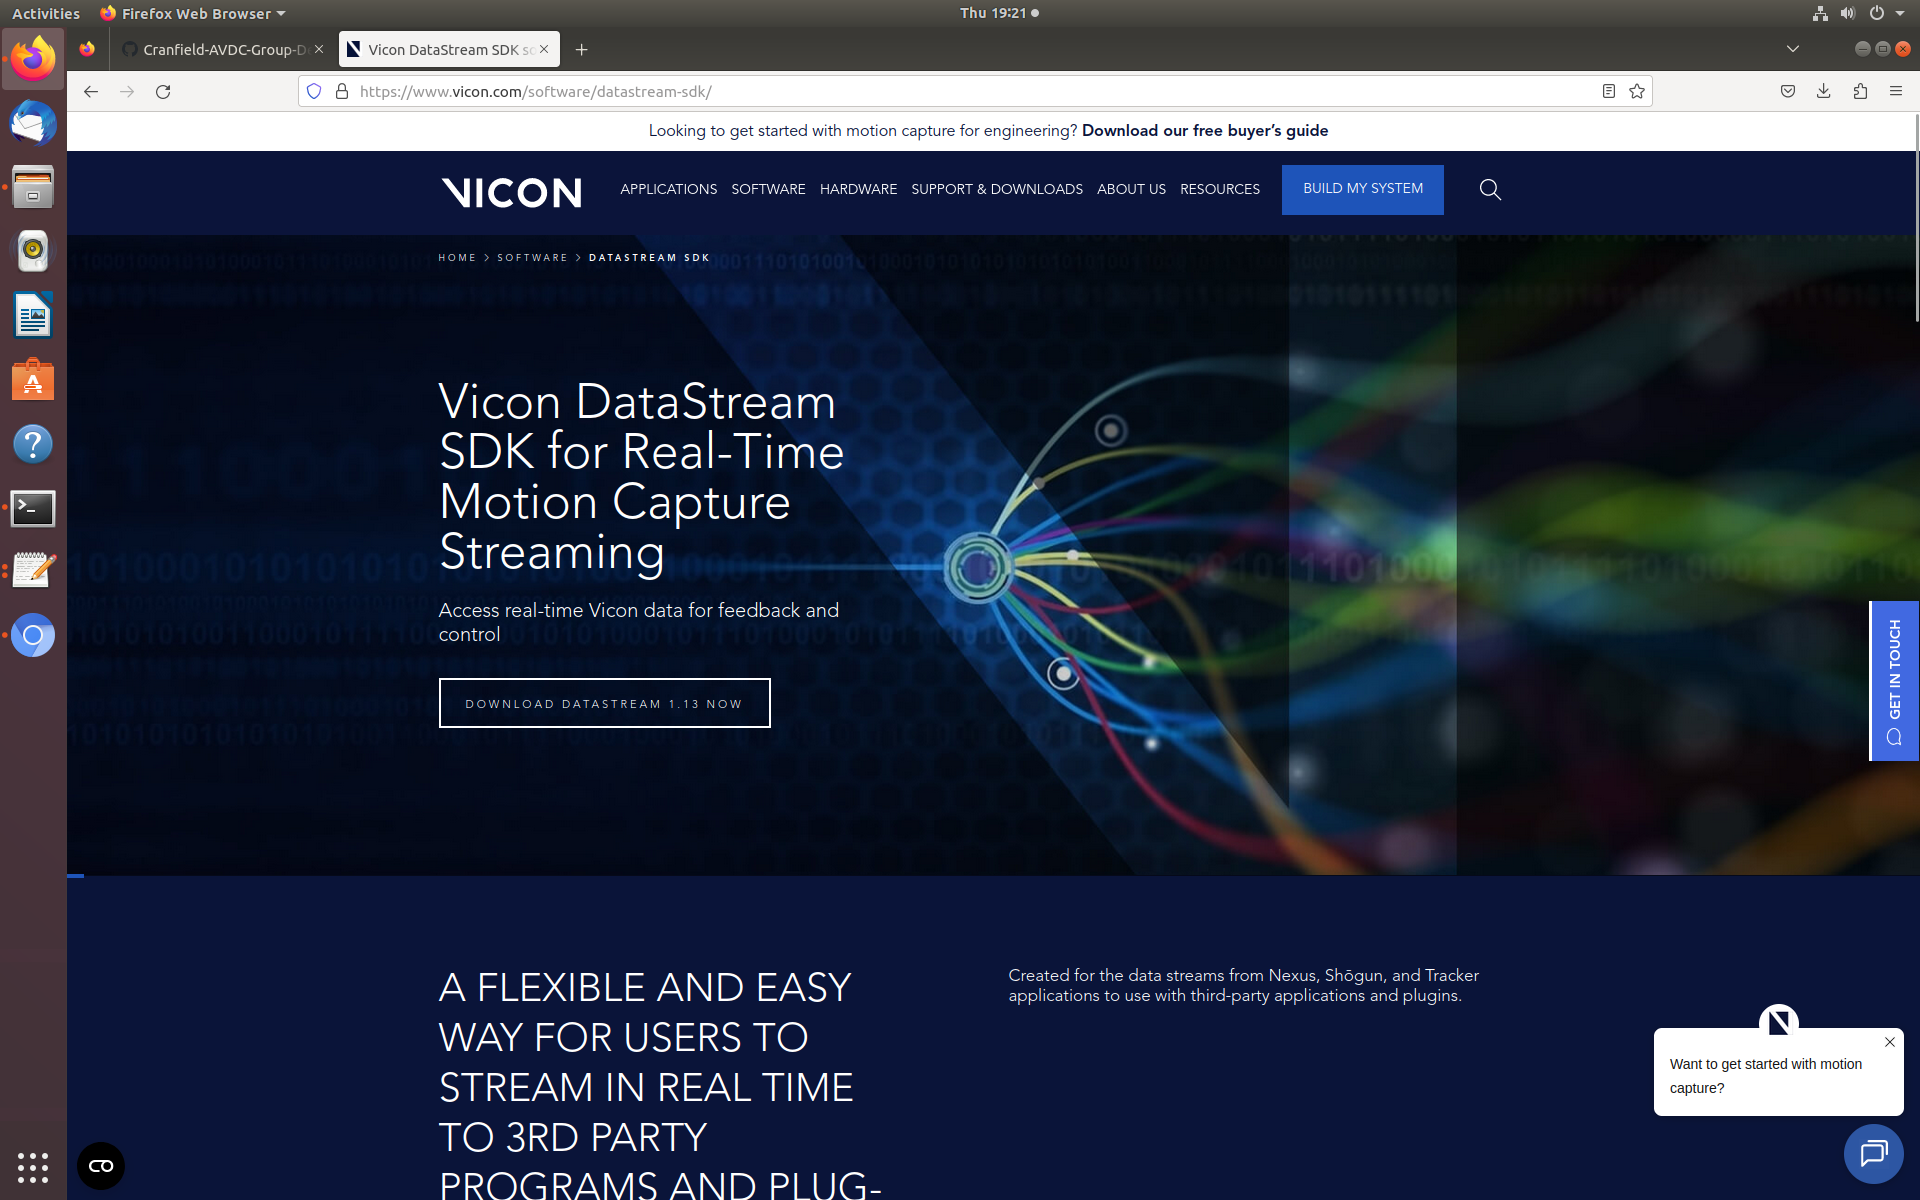
\includegraphics[width=0.9\linewidth]{Images/SDK1.png}
    \caption{VICON SDK Download Website}
    \label{fig:SDK1}
\end{figure}
Scroll down from the page to what is shown in figure \ref{fig:SDK2}:
\begin{figure}[H]
    \centering
    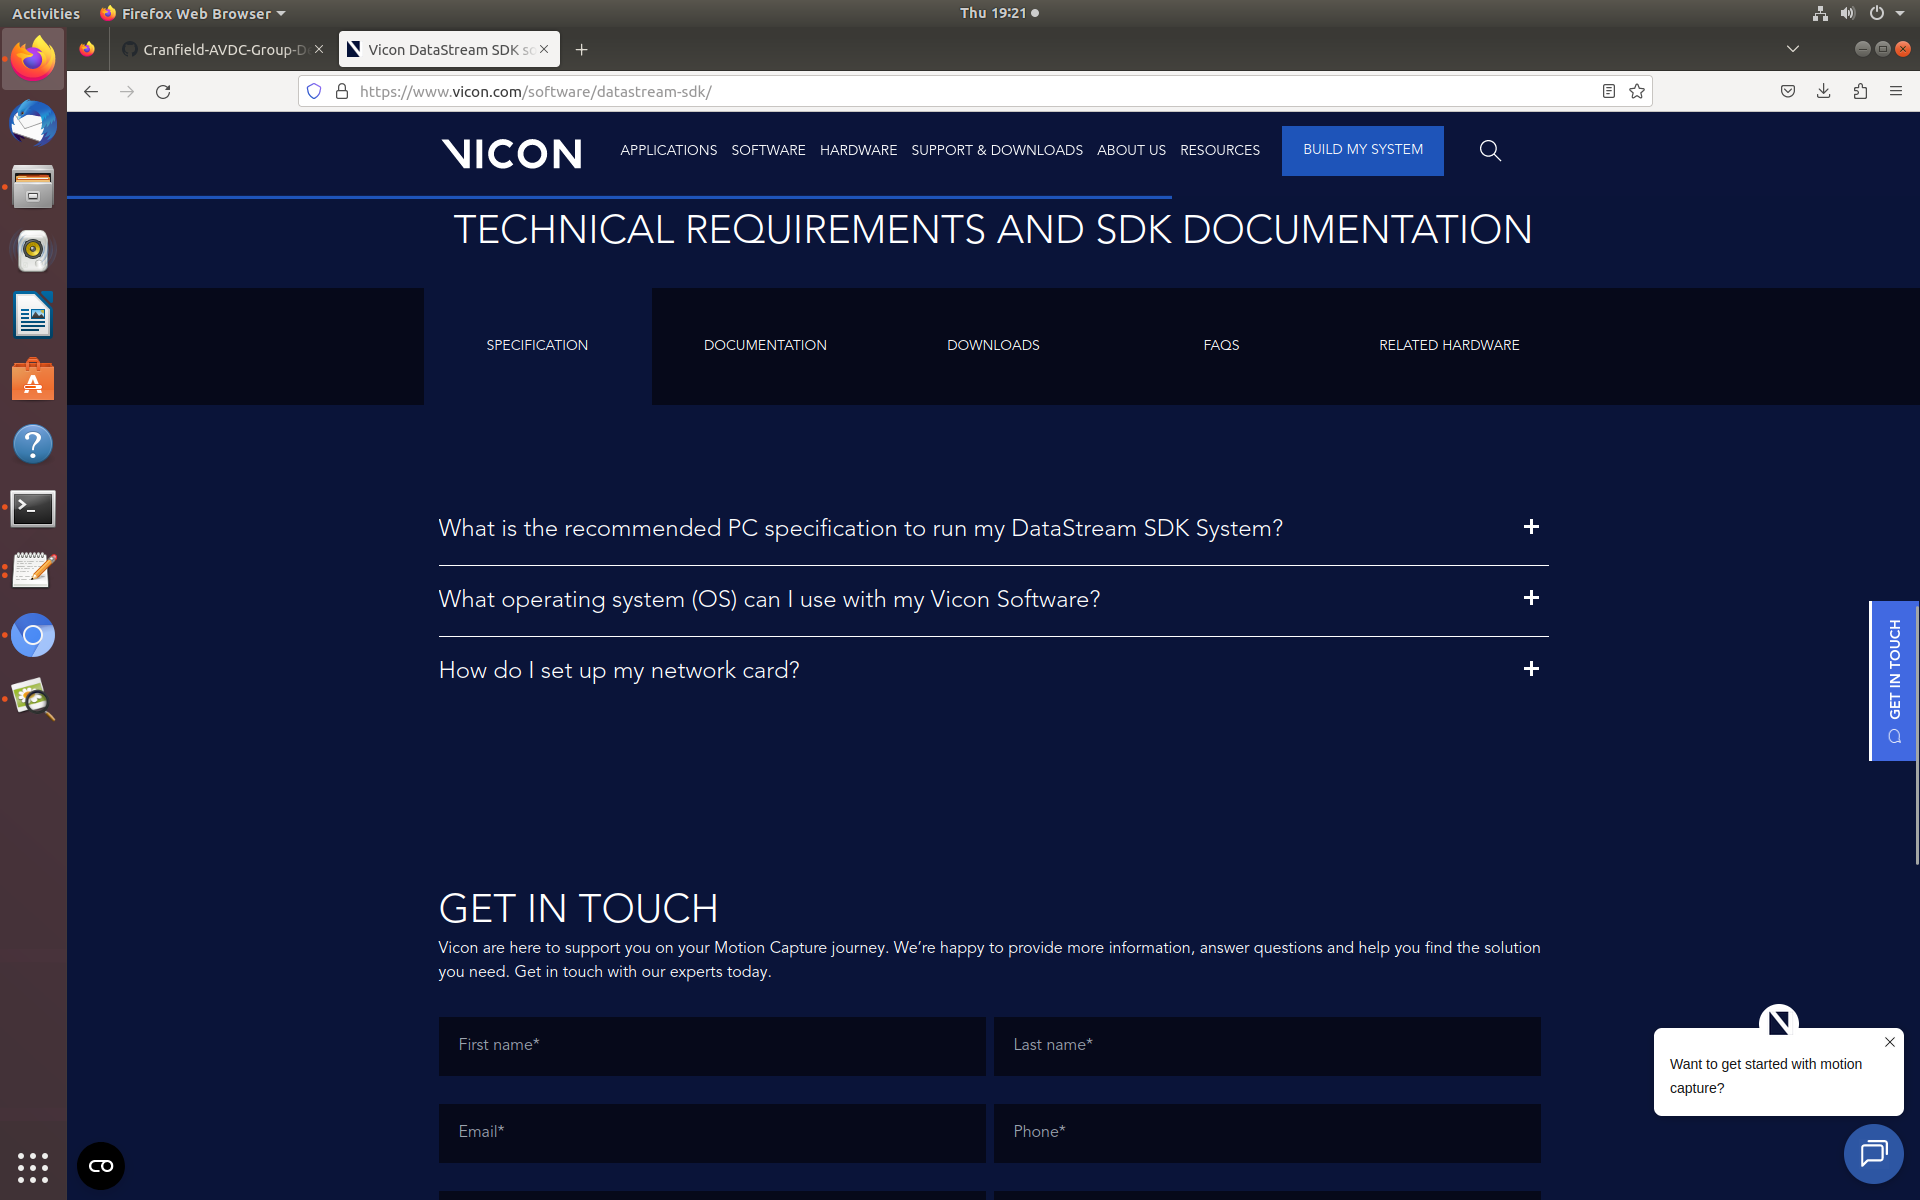
\includegraphics[width=1\linewidth]{Images/SDK2.png}
    \caption{VICON SDK Download Page}
    \label{fig:SDK2}
\end{figure}
Click the downloads tab, install the \textit{Datastream SDK 1.10.0}, write down \textit{an email}, \textit{No} for existing customer, \textit{Tracker} for the Software to Download, click \textit{DOWNLOAD}, as seen in figure \ref{fig:SDK3E}:
\begin{figure}[H]
    \centering
    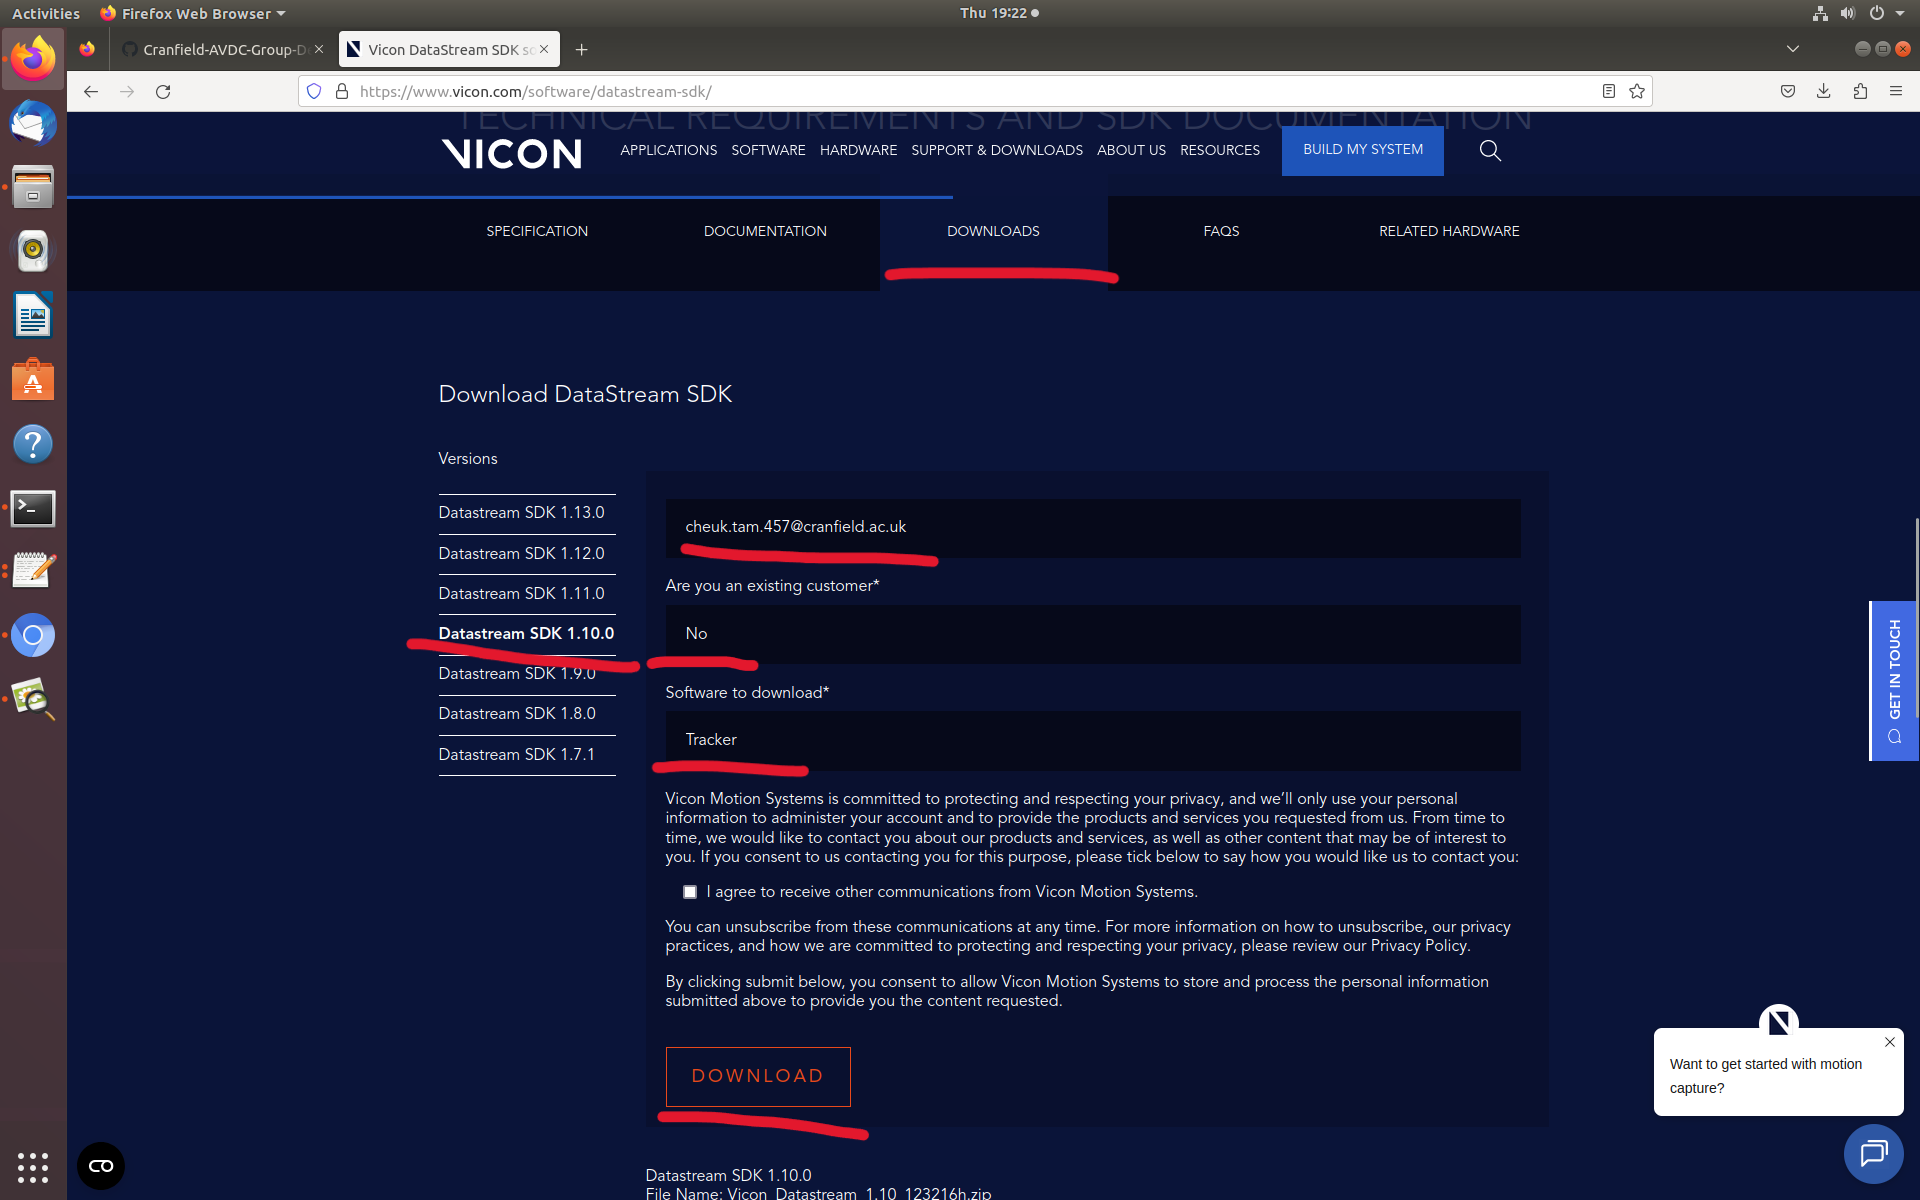
\includegraphics[width=0.9\linewidth]{Images/SDK3E.png}
    \caption{VICON SDK Download Information}
    \label{fig:SDK3E}
\end{figure}
Click \textit{Download} as seen in figure \ref{fig:SDK4}
\begin{figure}[H]
    \centering
    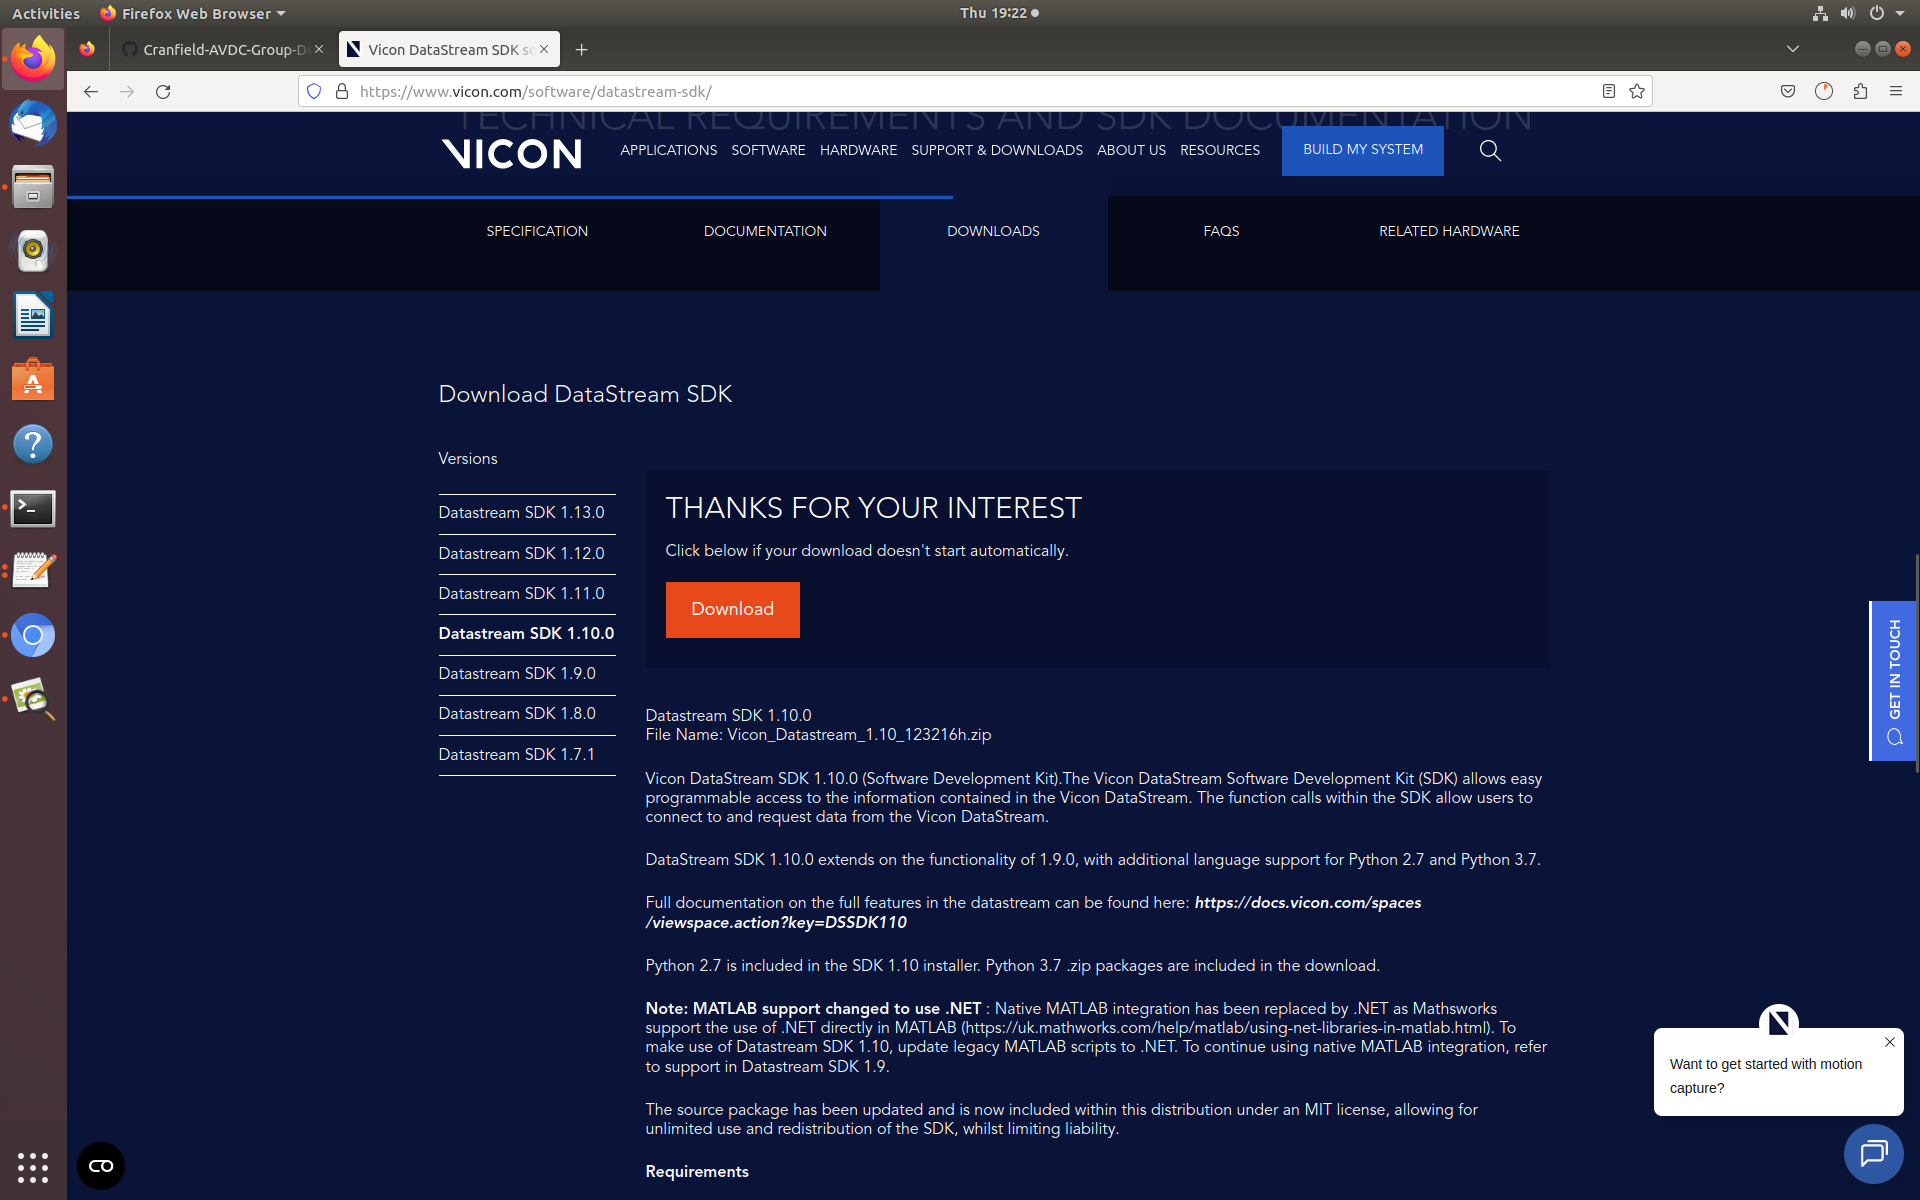
\includegraphics[width=1\linewidth]{Images/SDK4.png}
    \caption{VICON SDK Download}
    \label{fig:SDK4}
\end{figure}
Navigate to the your \textit{Downloads} Folder, click into \textit{Vicon\_Datastream\_1.10\_123216h.zip}, click into \textit{20200407\_123216h}, into \textit{Linux64}, into \textit{Release}, as seen in figure \ref{fig:SDK59}
\begin{figure}[H]
    \centering
    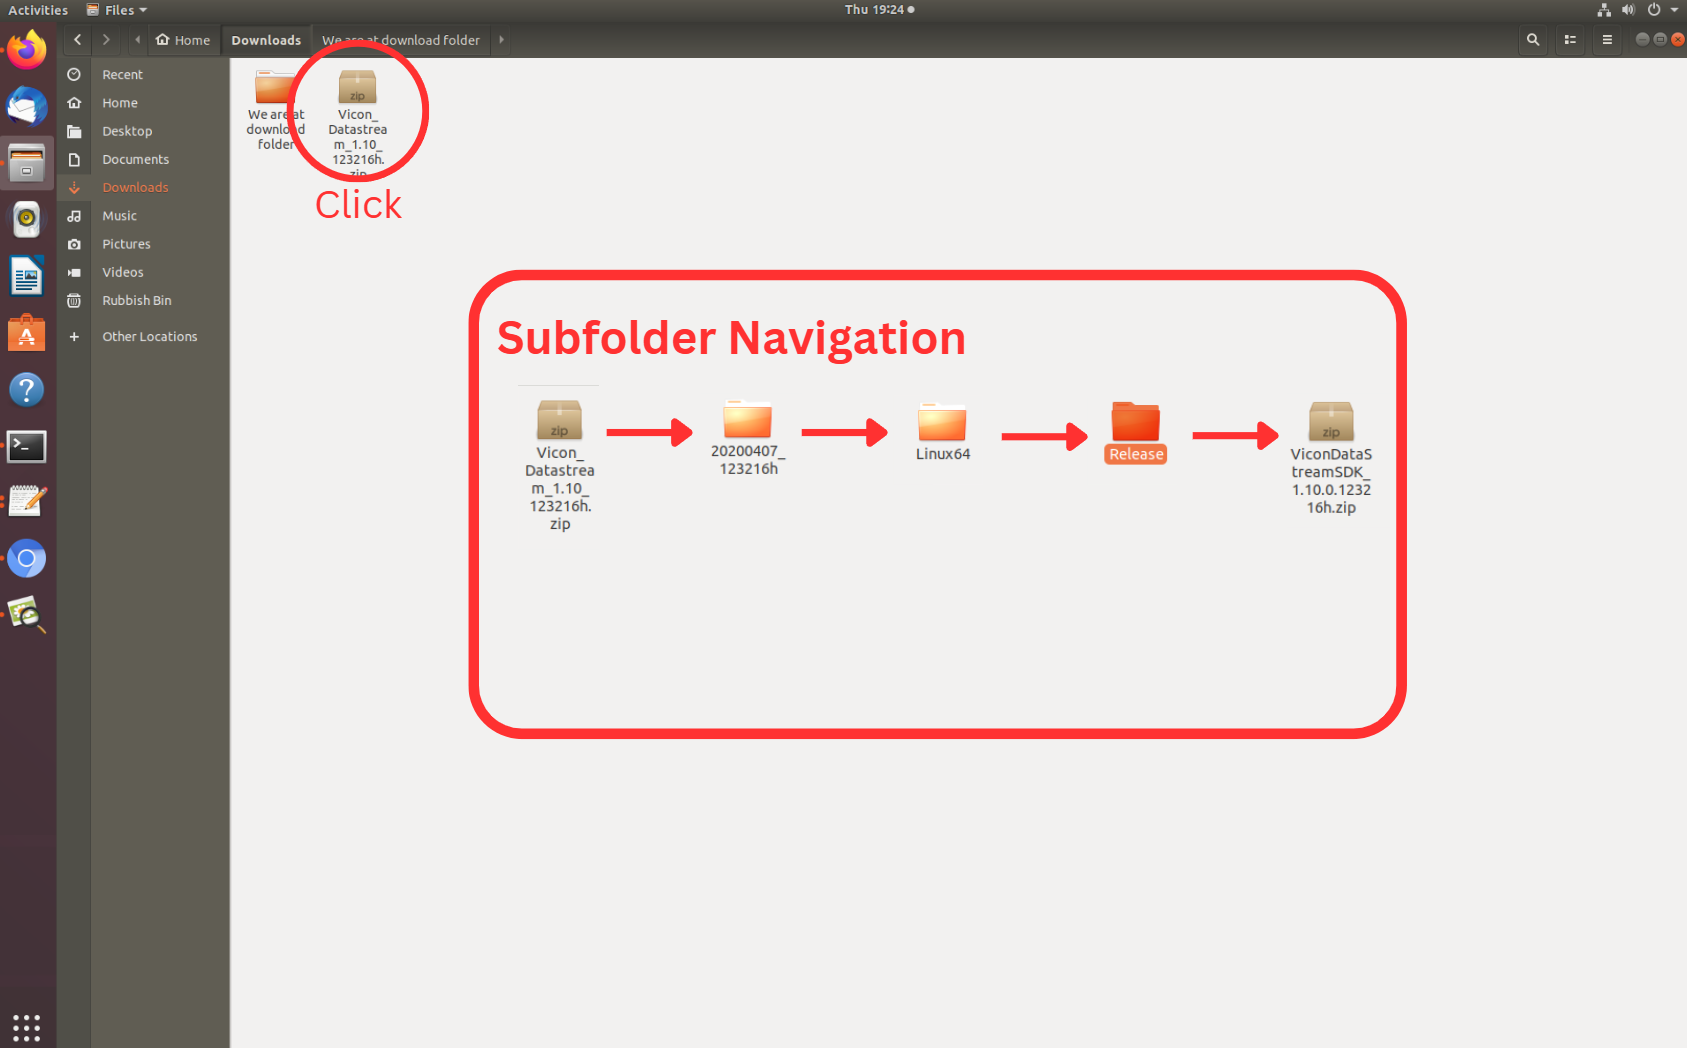
\includegraphics[width=0.9\linewidth]{Images/SDK59.png}
    \caption{Navigate to Linux64/Release inside Vicon SDK}
    \label{fig:SDK59}
\end{figure}
Right click on \textit{ViconDataStreamSDK\_1.10.0.123216h.zip}, extract the file, you should have a file like figure \ref{fig:SDK9}
\begin{figure}[H]
    \centering
    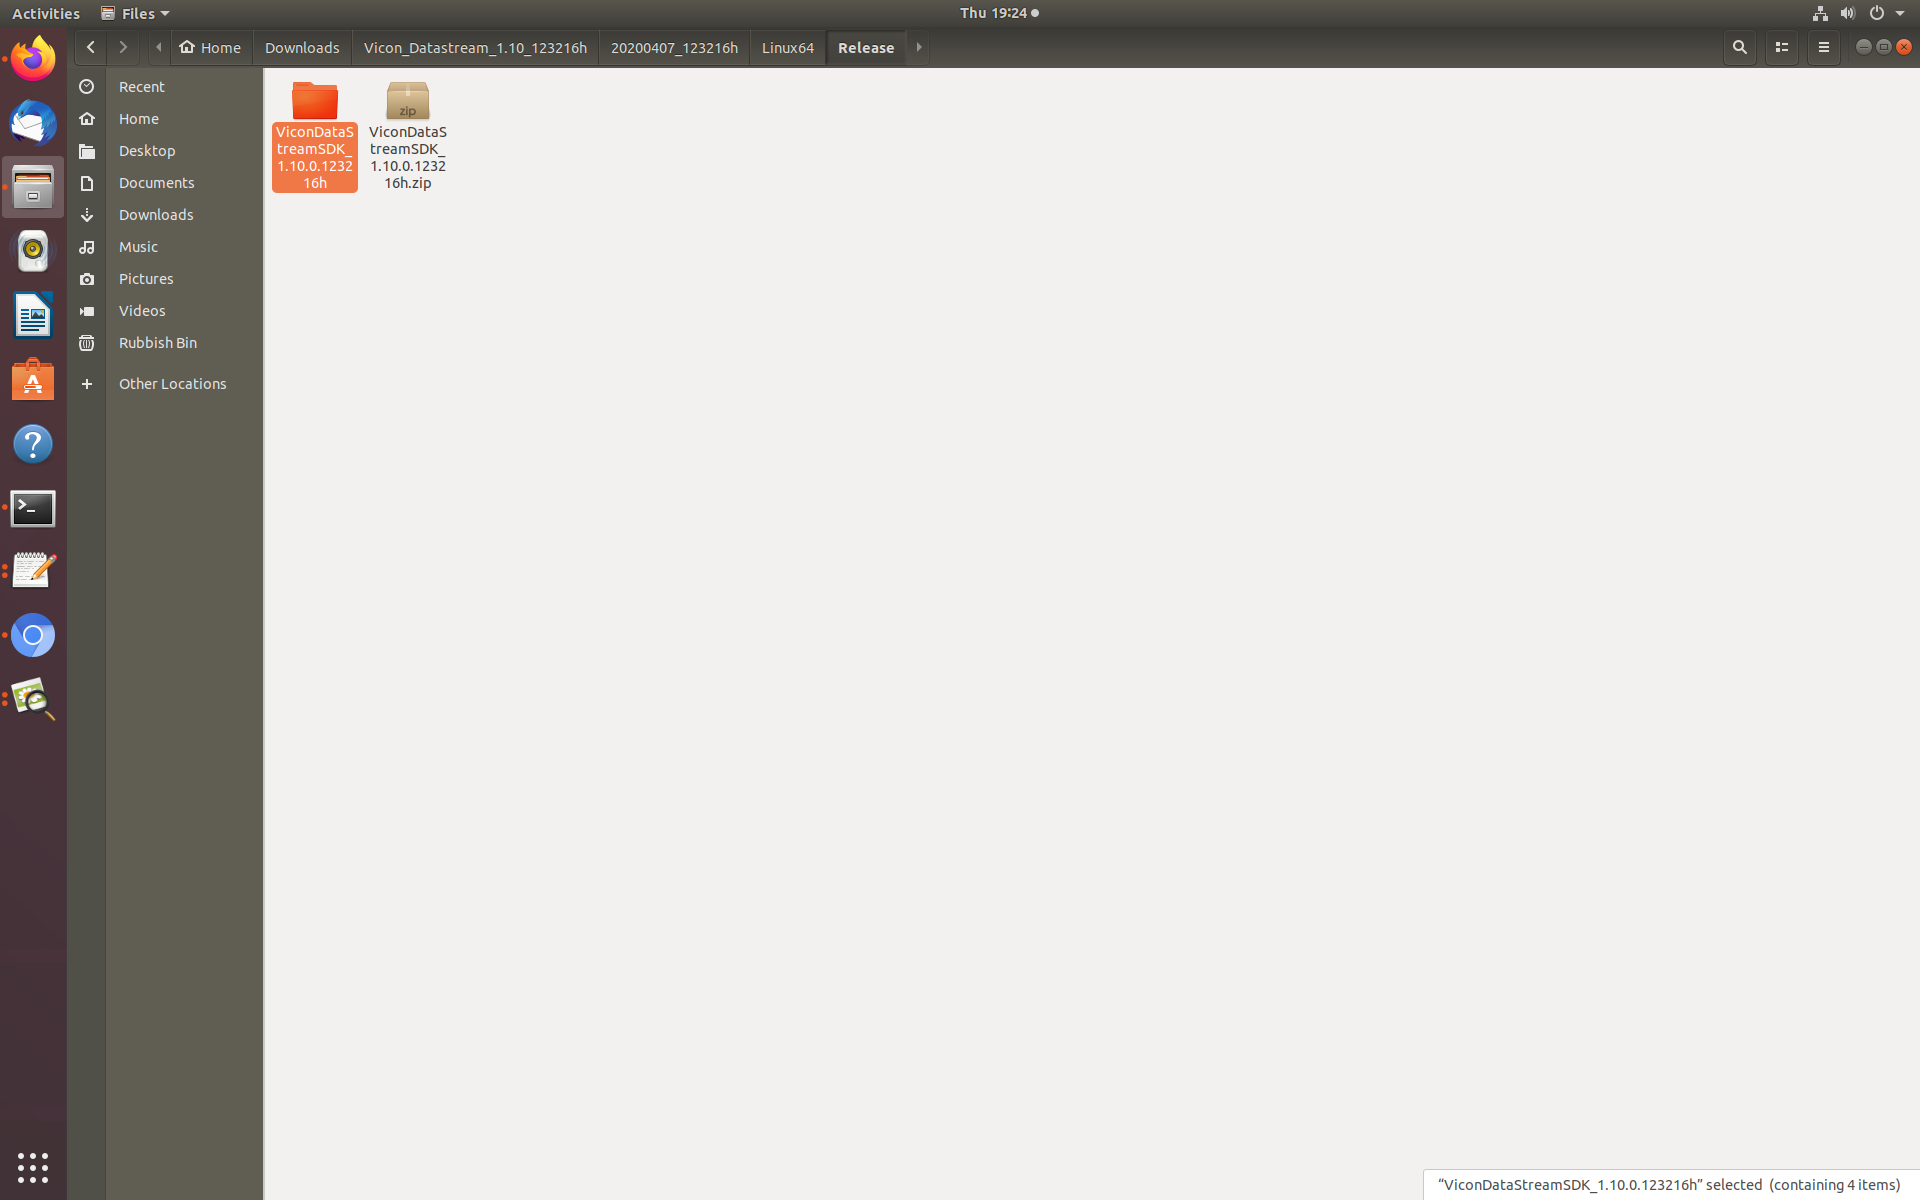
\includegraphics[width=1\linewidth]{Images/SDK9.png}
    \caption{Extracted file of Linux64 Vicon SDK}
    \label{fig:SDK9}
\end{figure}
Drag the extracted file of the Vicon SDK back to the download dictionary as shown in figure \ref{fig:SDK10}
\begin{figure}[H]
    \centering
    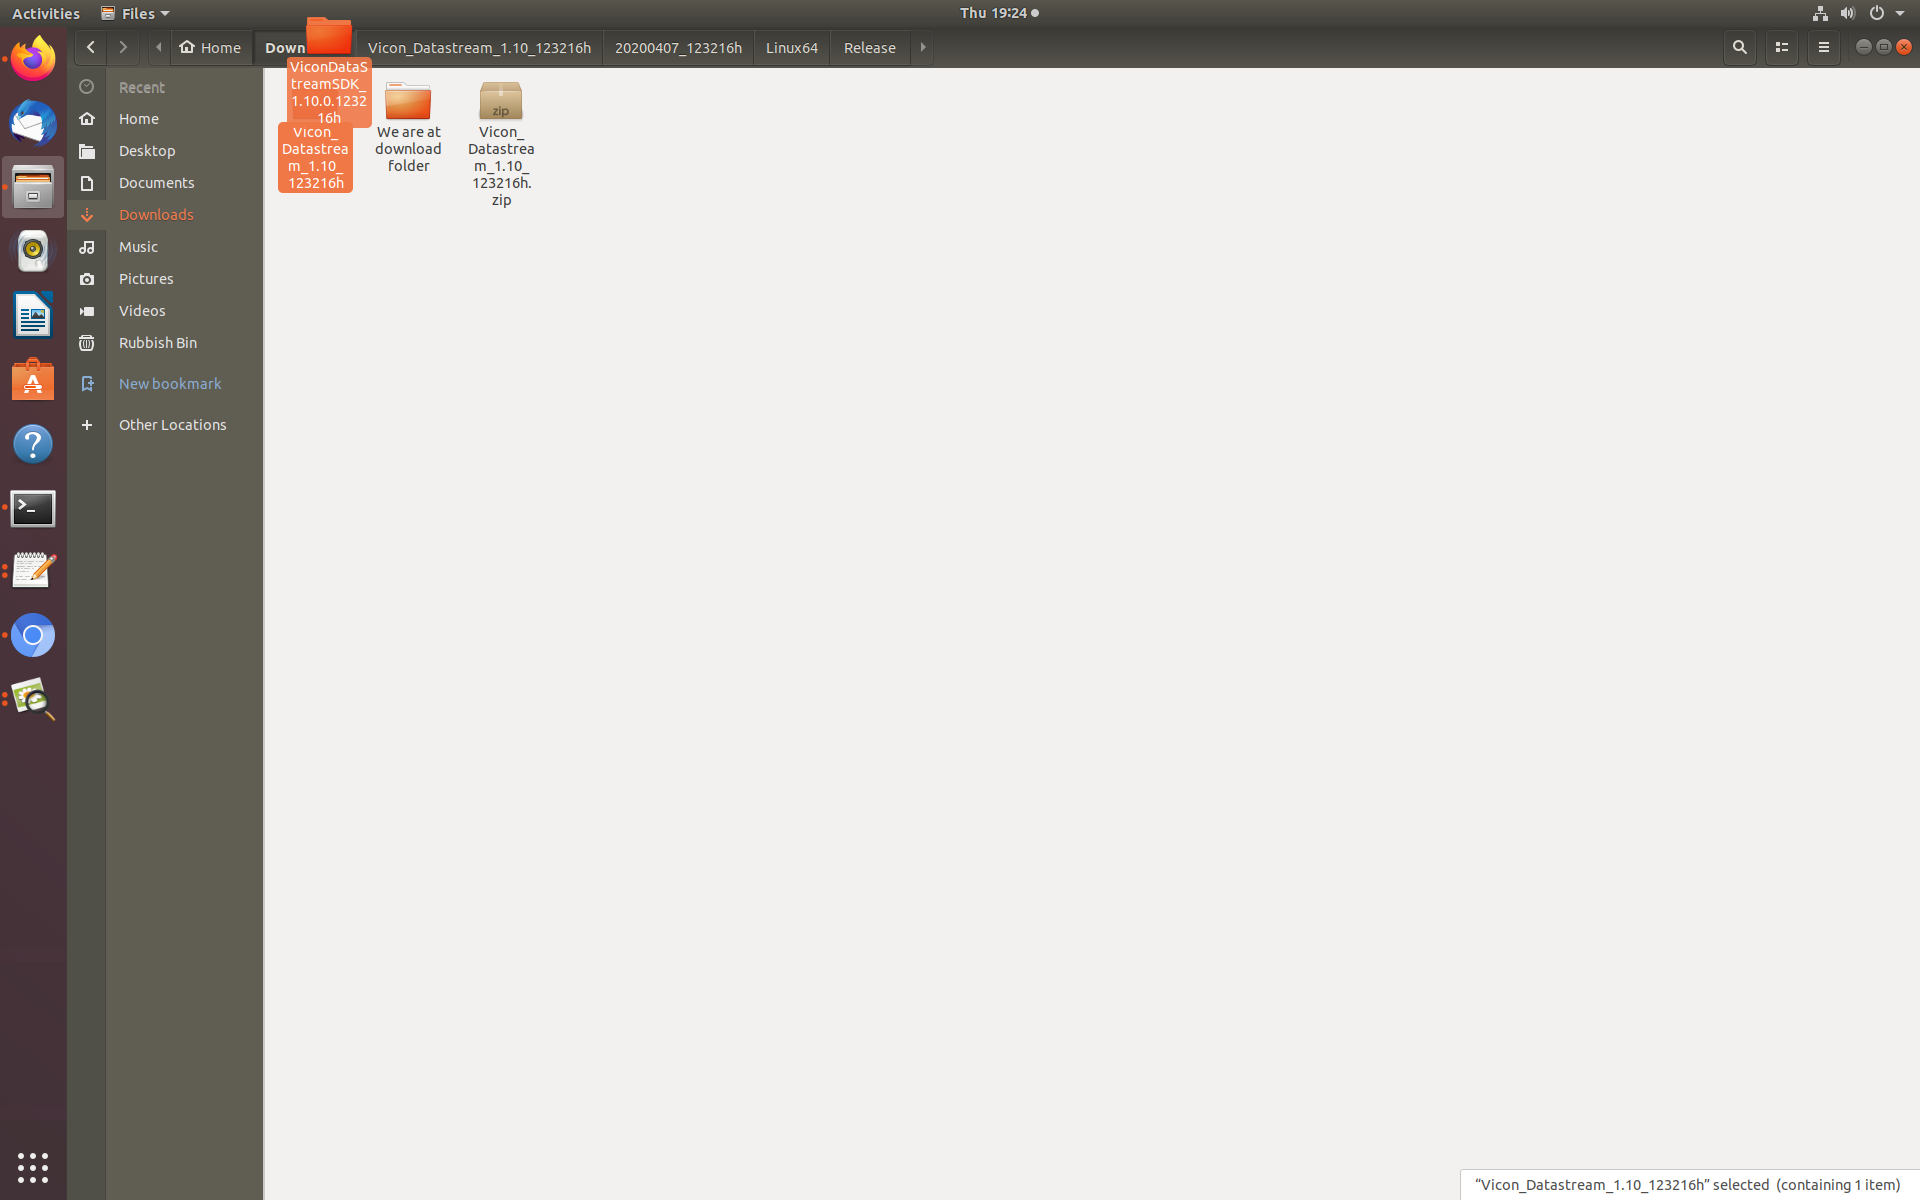
\includegraphics[width=0.9\linewidth]{Images/SDK10.png}
    \caption{Moving Vicon SDK into download folders}
    \label{fig:SDK10}
\end{figure}
Remove the original zip file, they are no longer needed, you should have a singular file as shown in figure \ref{fig:SDK11}.
\begin{figure}[H]
    \centering
    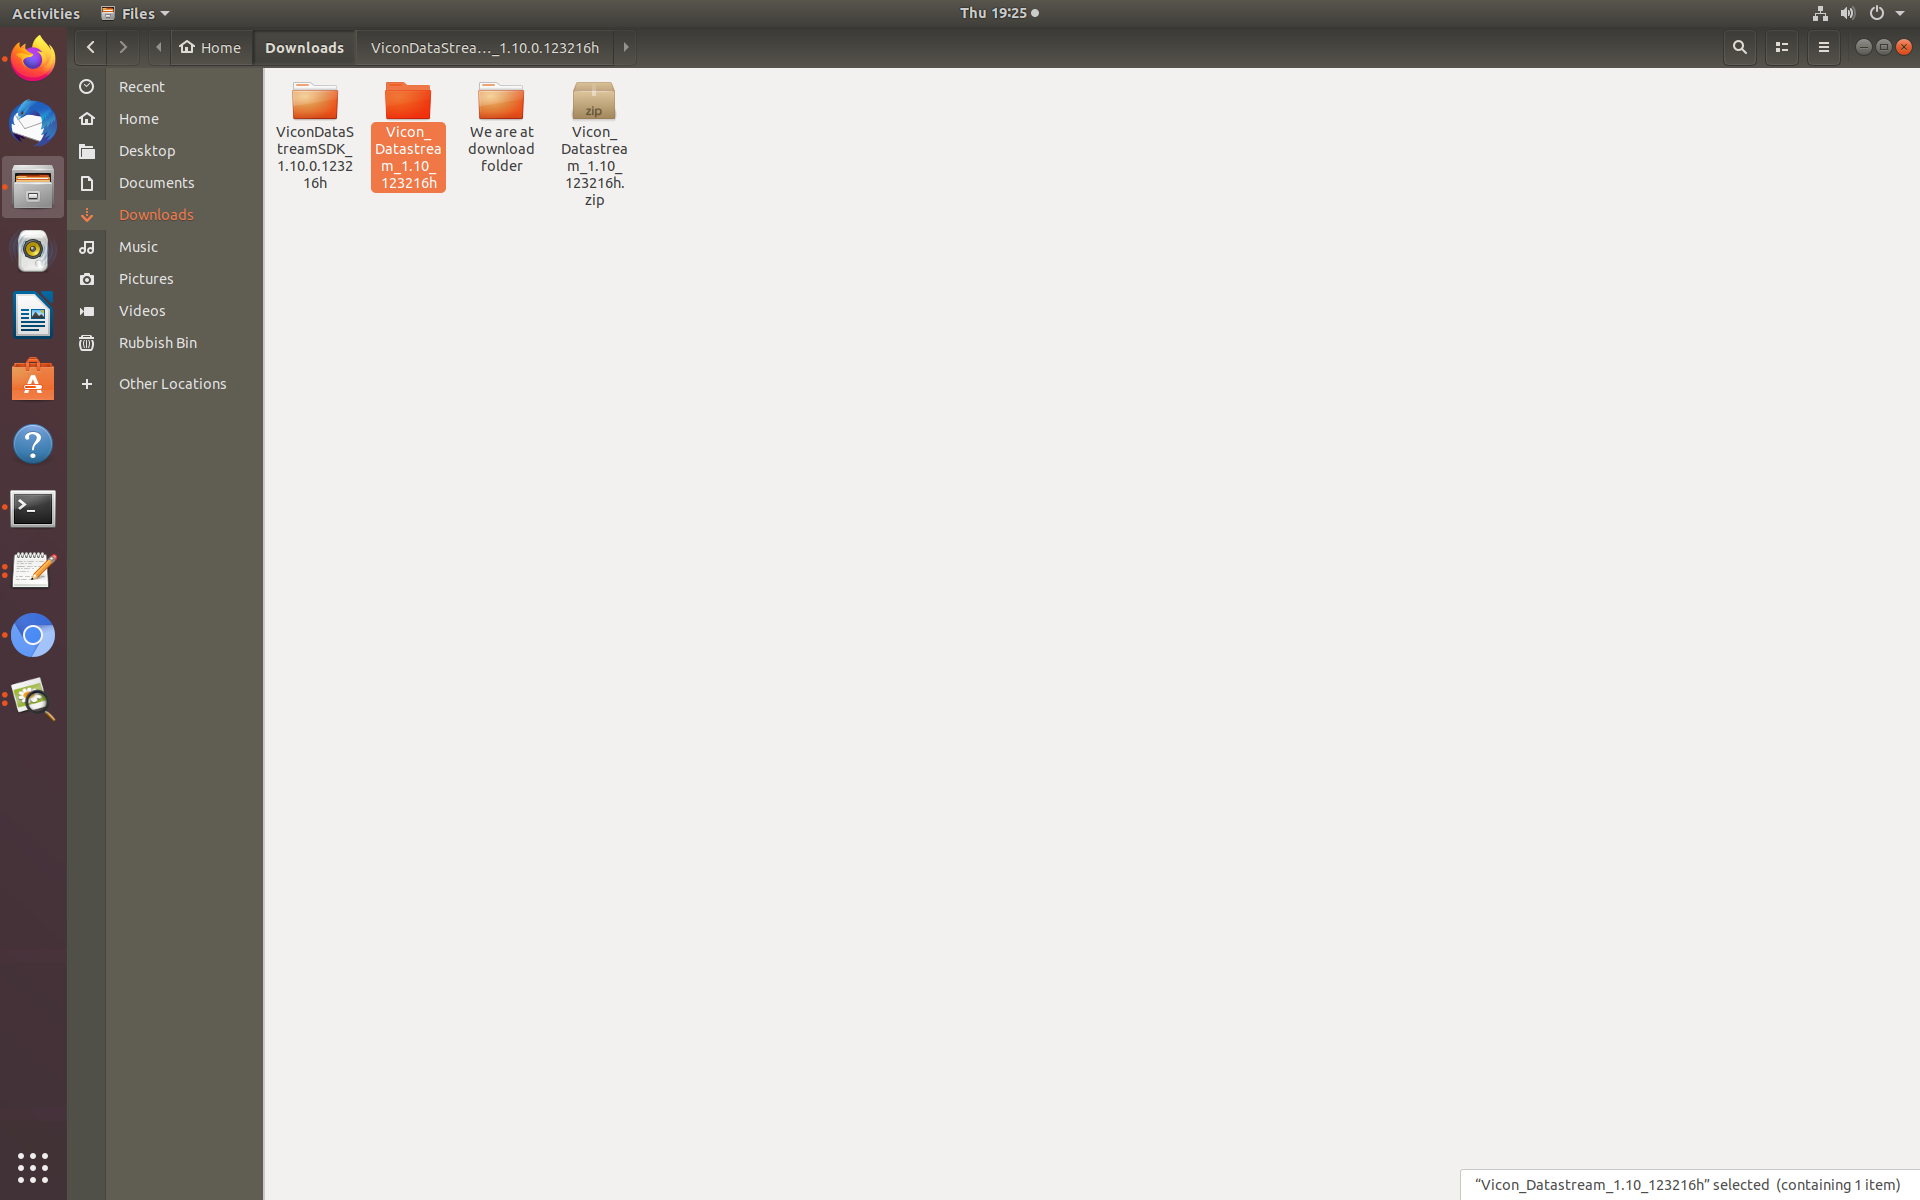
\includegraphics[width=1\linewidth]{Images/SDK11.png}
    \caption{Linux64 Vicon SDK extracted in Downloads Folder}
    \label{fig:SDK11}
\end{figure}
Click into the SDK folder (\textit{ViconDataStreamSDK\_1.10.0.123216h}), you should see 2 zipped files inside it like figure \ref{fig:SDK14}.
\begin{figure}[H]
    \centering
    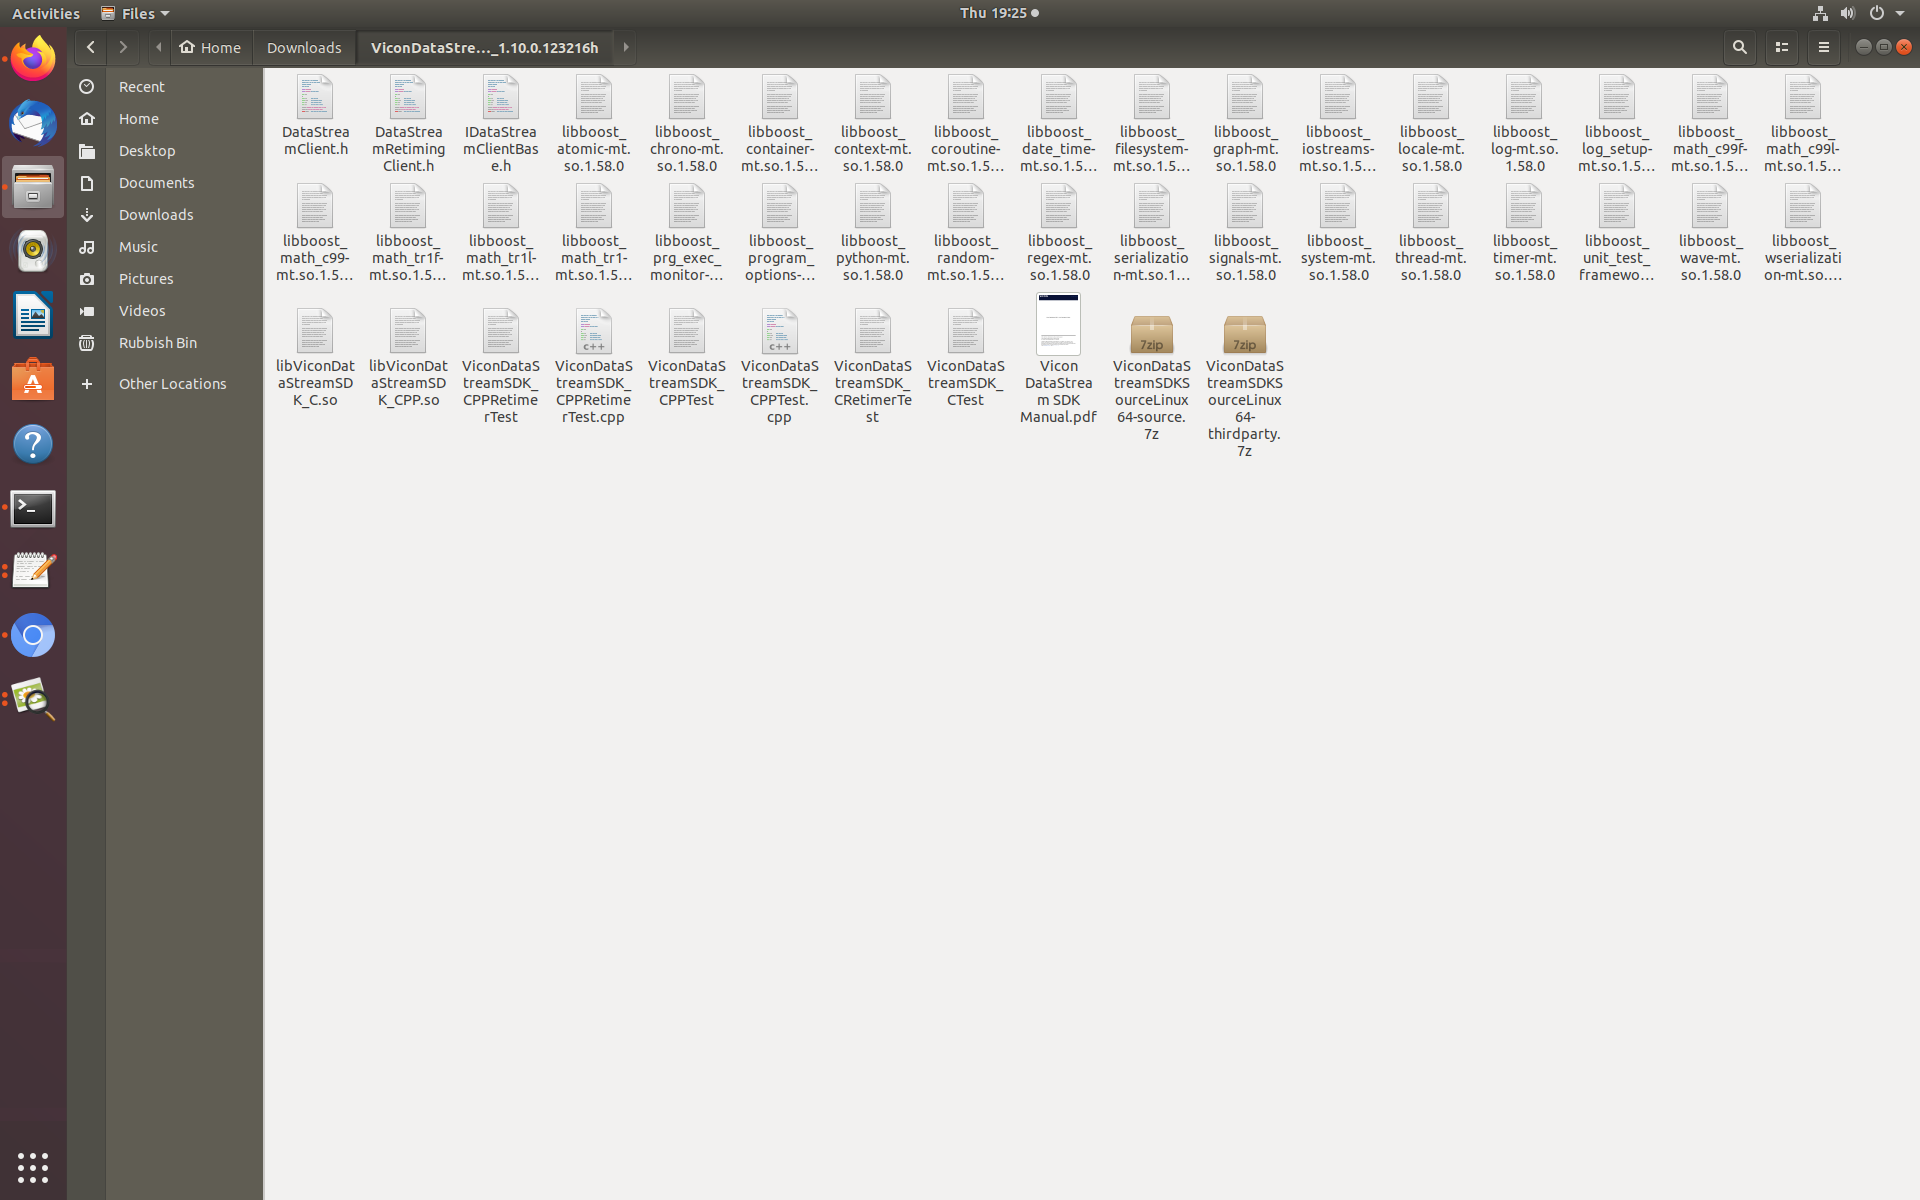
\includegraphics[width=1\linewidth]{Images/SDK14.png}
    \caption{Vicon SDK Folder}
    \label{fig:SDK14}
\end{figure}
Extract the 2 zipped files as shown in figure \ref{fig:SDK15}.
\begin{figure}[H]
    \centering
    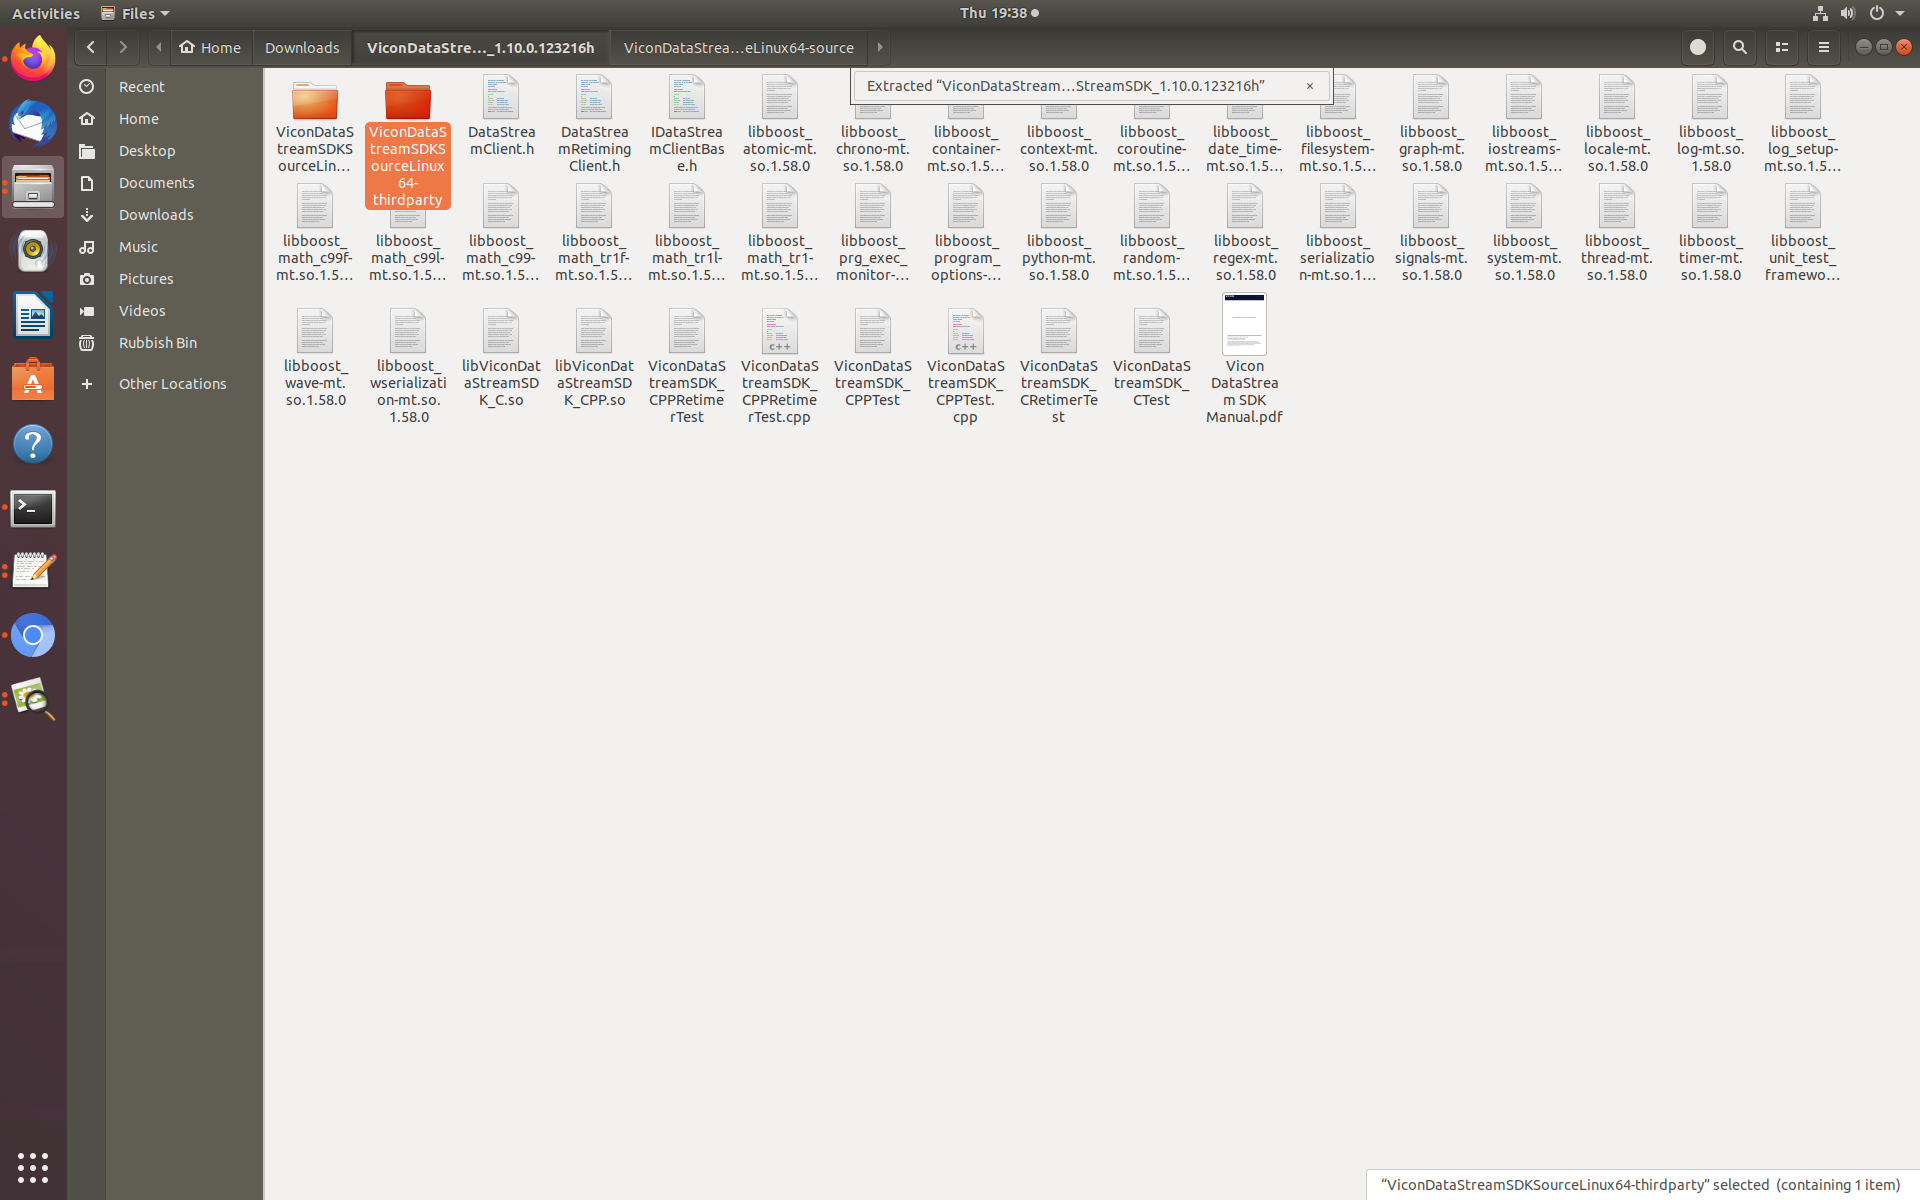
\includegraphics[width=1\linewidth]{Images/SDK15.png}
    \caption{Extracted 2 Subfolders of Vicon SDK Folder}
    \label{fig:SDK15}
\end{figure}

\subsection{Downloading pyvicon}
After SDK is installed, you will need install a custom python script by MathGaron \cite{pyvicon} that bridges the VICON SDK to MAVPROXY. This is installed via
 \href{https://github.com/MathGaron/pyvicon}{https://github.com/MathGaron/pyvicon}, as seen in figure \ref{fig:SDK155}:
 \begin{figure}[H]
     \centering
     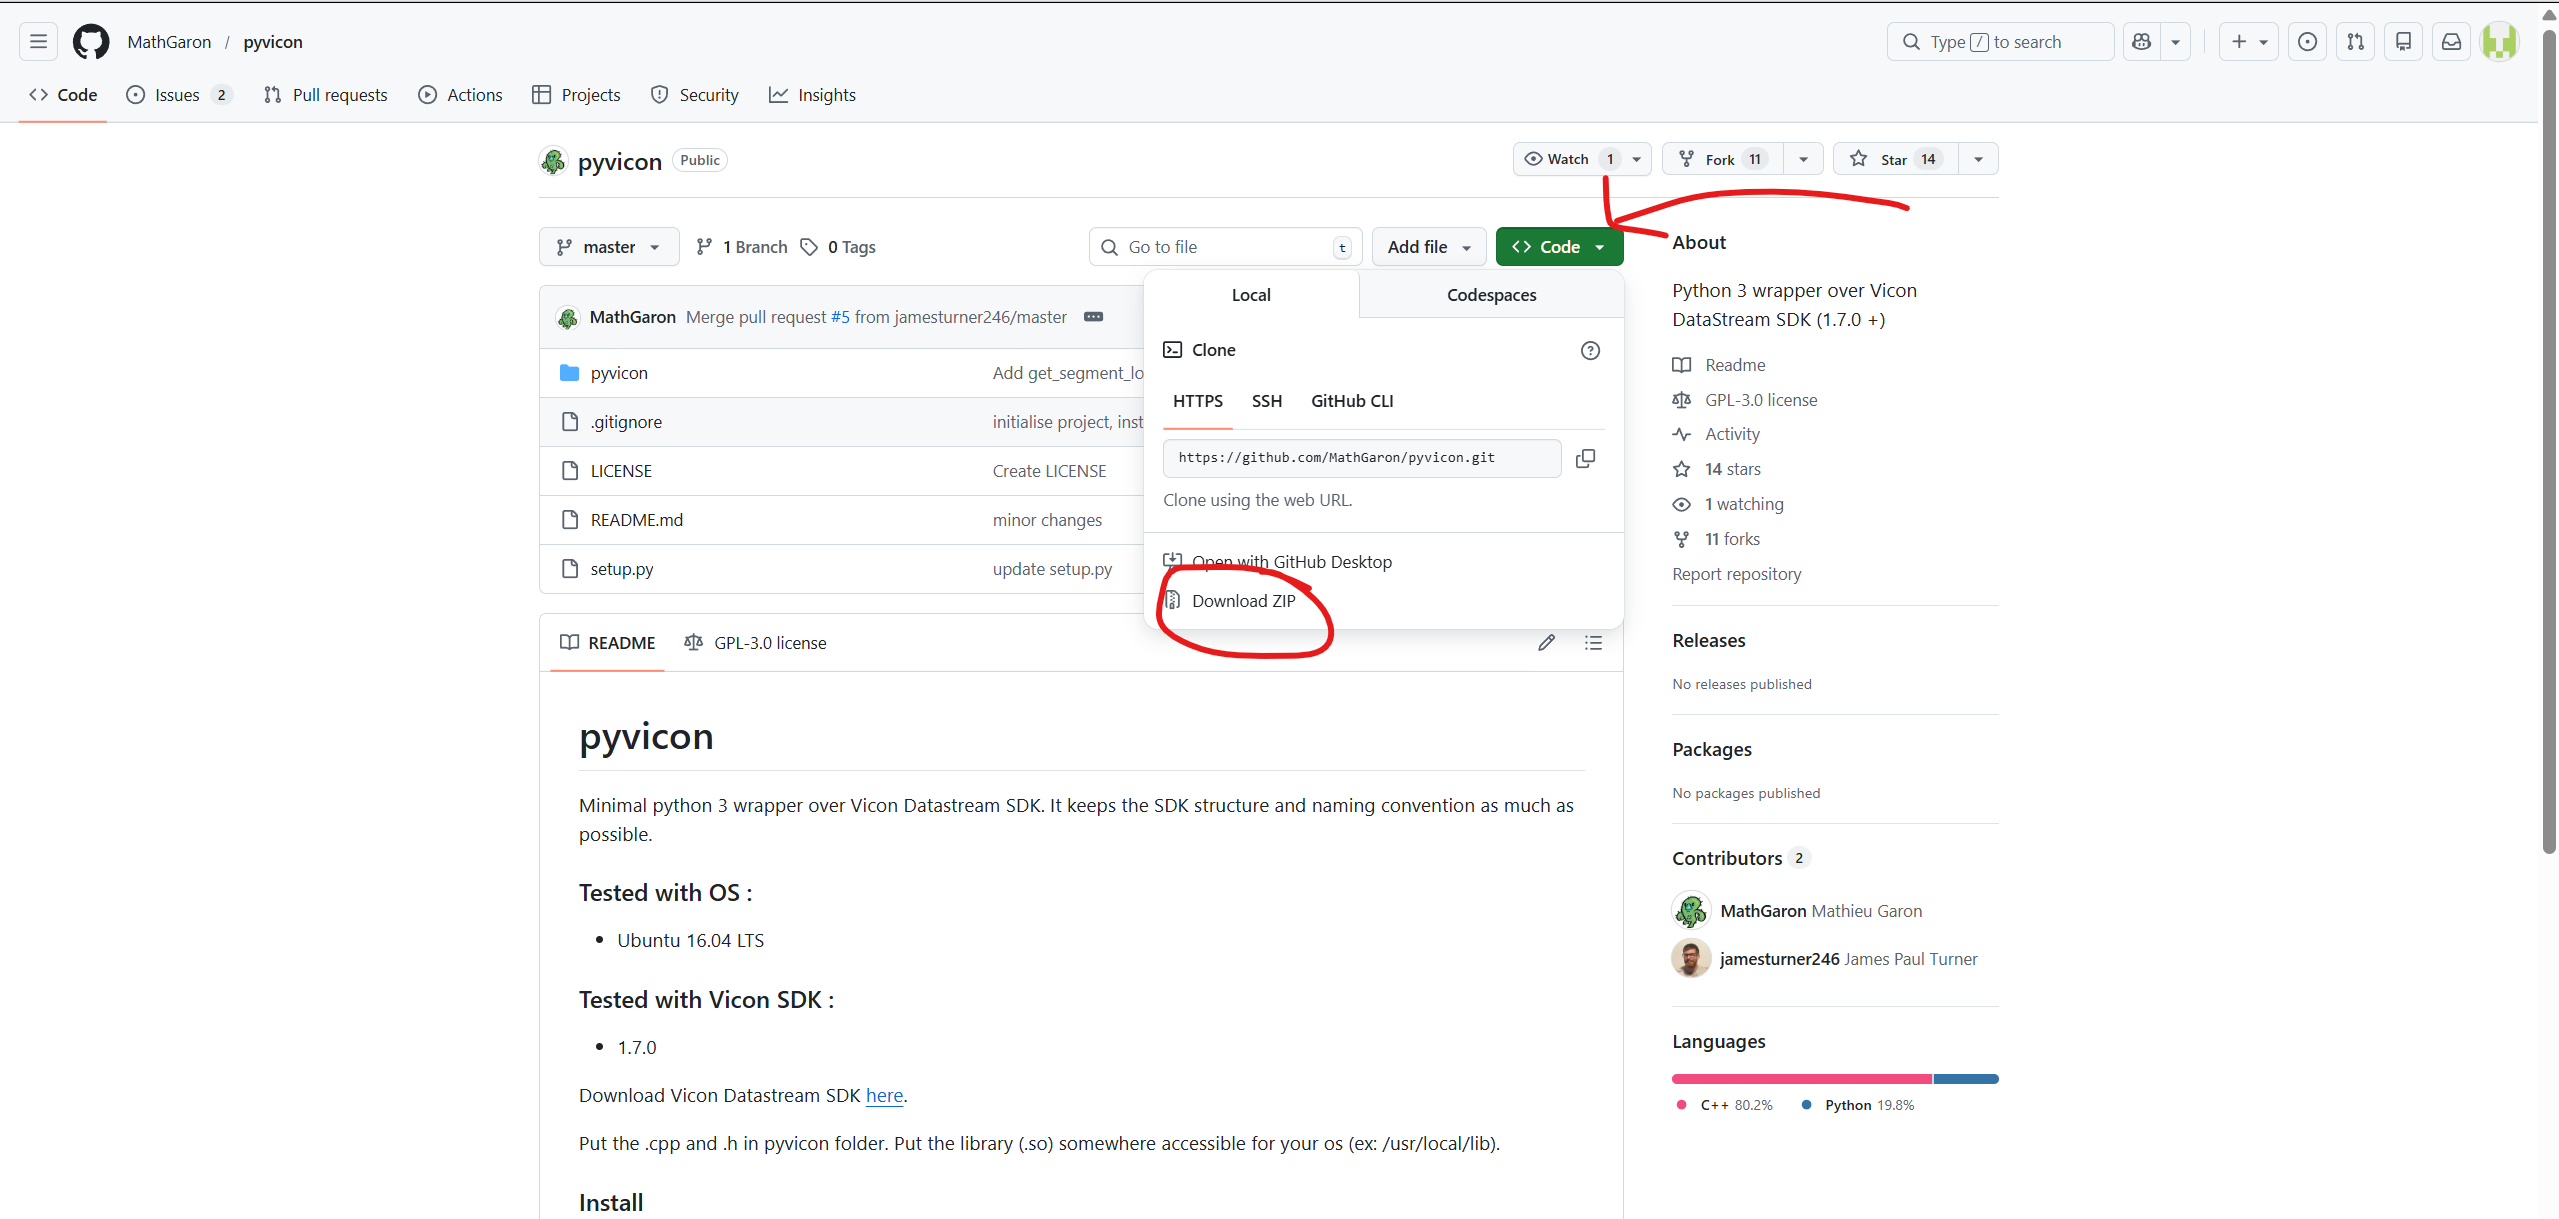
\includegraphics[width=1\linewidth]{Images/SDK155.png}
     \caption{Install the Github file. (Click \textit{Code}, and \textit{Download Zip})}
     \label{fig:SDK155}
\end{figure}
Extract the zipped pyvicon folder into your download folders. Your donwload folder should now have the Vicon SDK folder \& pyvicon folder, as seen in figure \ref{fig:pyvicon1}: 
\begin{figure}[H]
    \centering
    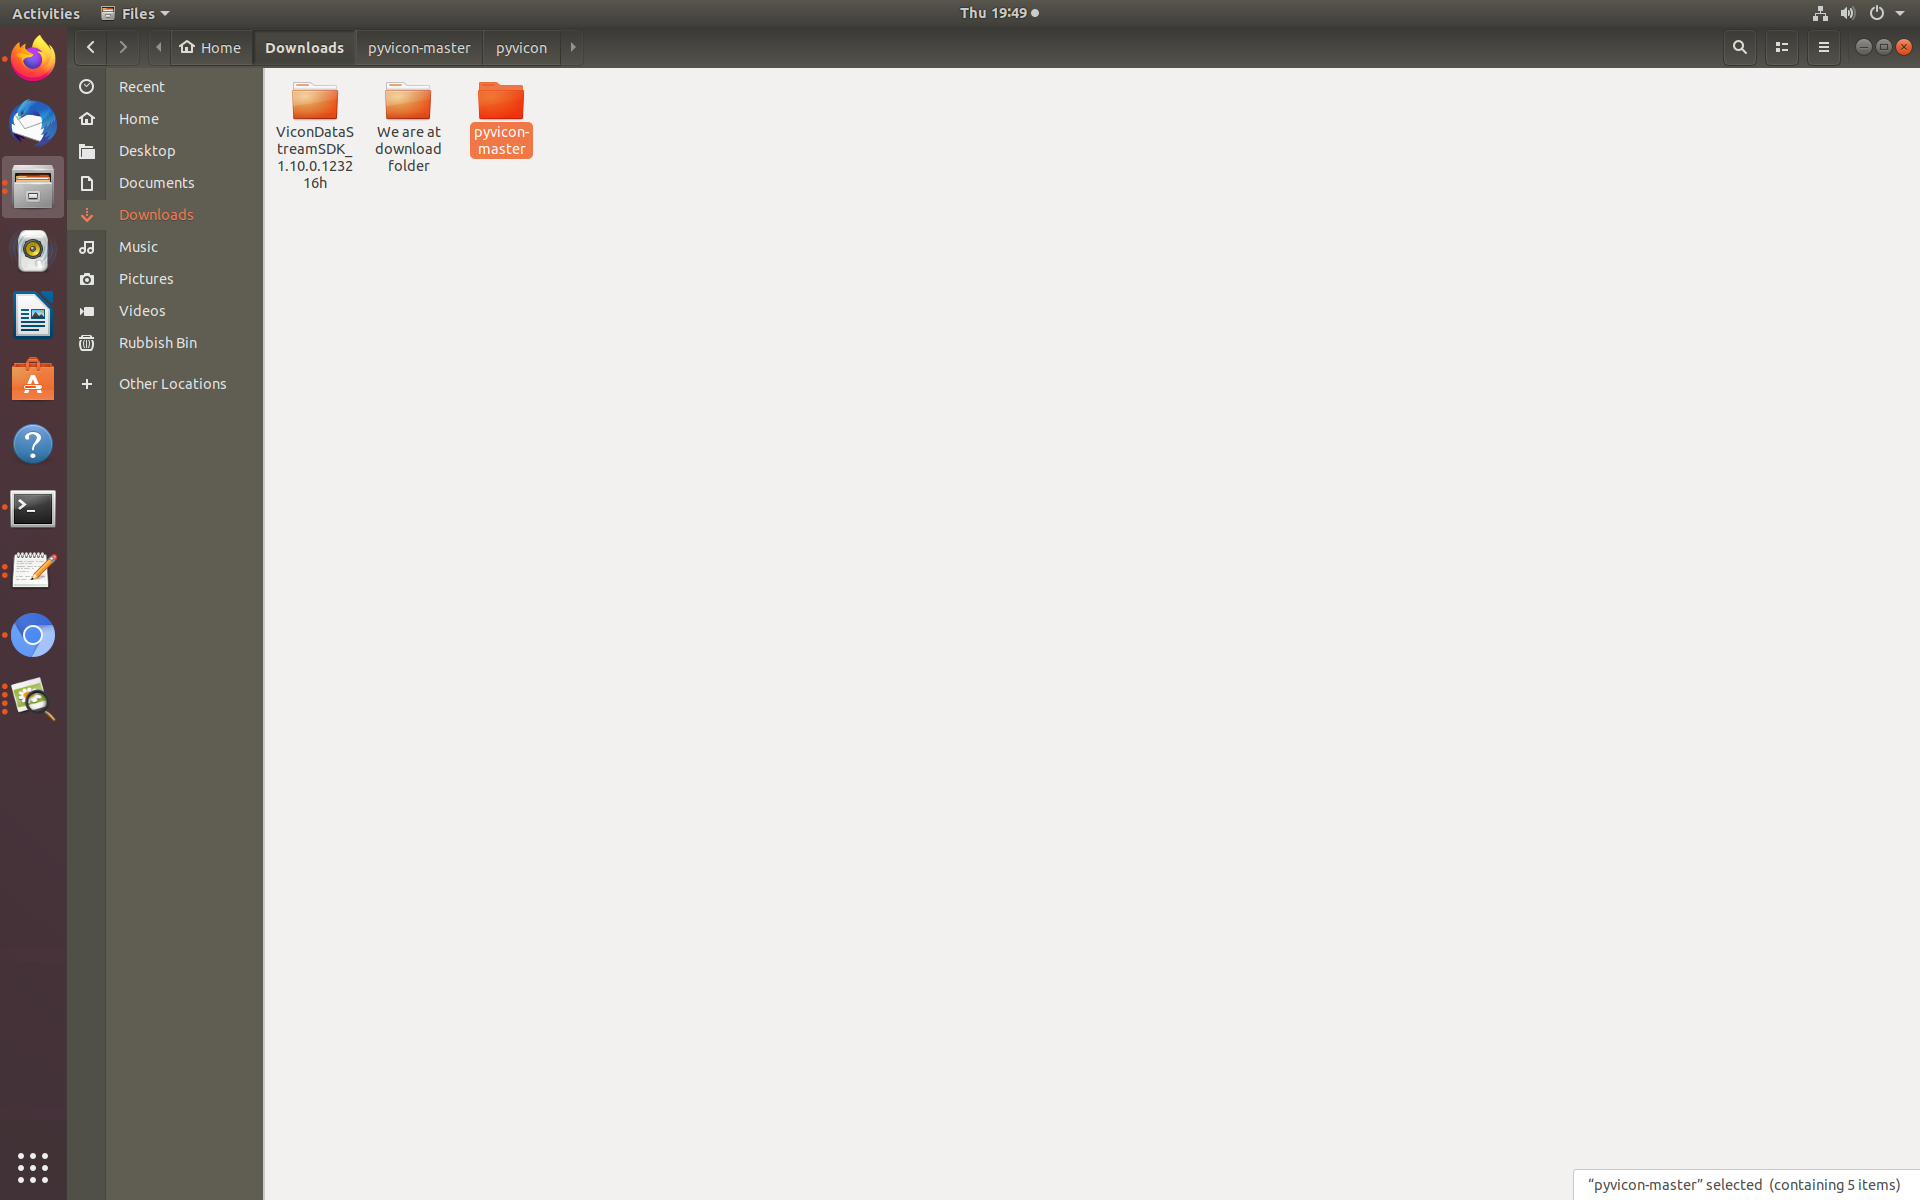
\includegraphics[width=1\linewidth]{Images/pyvicon1.png}
    \caption{Vicon SDK folder and pyvicon folder in Downloads Folder}
    \label{fig:pyvicon1}
\end{figure}
\subsection{Merging VICON SDK into pyvicon}
Next, you need to merge the .so files of the VICON SDK into your venv's lib directory. Run these following code in your terminal, as seen in figure \ref{fig:SDK1555}: \\
\begin{figure}[H]
    \centering
    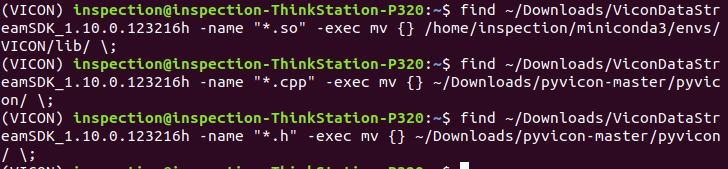
\includegraphics[width=1\linewidth]{Images/VirtualEnvironment/Five.png}
    \caption{Three scripts to merge SDK into venv's lib folder and setting up pyvicon.}
    \label{fig:SDK1555}
\end{figure}
The first of the three commands above moves all the .so files from the Vicon SDK folder into your venv's lib folder, which is usually located in \textit{miniconda3/envs/VICON/lib}.:
\begin{lstlisting}
find ~/Downloads/ViconDataStreamSDK_1.10.0.123216h -name "*.so" -exec mv {} /home/inspection/miniconda3/envs/VICON/lib/ \;
\end{lstlisting}

Your \textit{miniconda3/envs/VICON/lib} folder should now have the .so files of Vicon SDK, it should look like figure \ref{fig:SDK16}:
\begin{figure}[H]
    \centering
    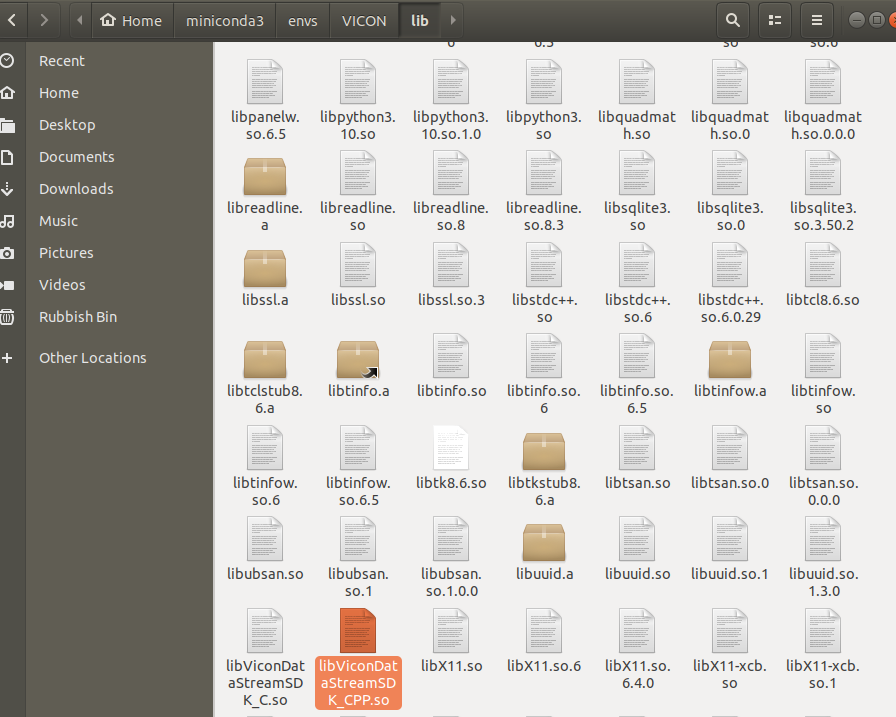
\includegraphics[width=1\linewidth]{Images/VirtualEnvironment/Three.png}
    \caption{.so files of Vicon SDK merged into venv's lib folder}
    \label{fig:SDK16}
\end{figure}

The 2nd and 3rd commands move the .cpp and .h files of ViconDataStreamSDK into pyvicon-master/pyvicon:
\begin{lstlisting}
find ~/Downloads/ViconDataStreamSDK_1.10.0.123216h -name "*.cpp" -exec mv {} ~/Downloads/pyvicon-master/pyvicon/ \; 
\end{lstlisting}
\begin{lstlisting}
find ~/Downloads/ViconDataStreamSDK_1.10.0.123216h -name "*.h" -exec mv {} ~/Downloads/pyvicon-master/pyvicon/ \;
\end{lstlisting}
The pyvicon folder should now have the .cpp and .h files of Vicon SDK like in figure \ref{fig:SDK17}:
\begin{figure}[H]       
    \centering
    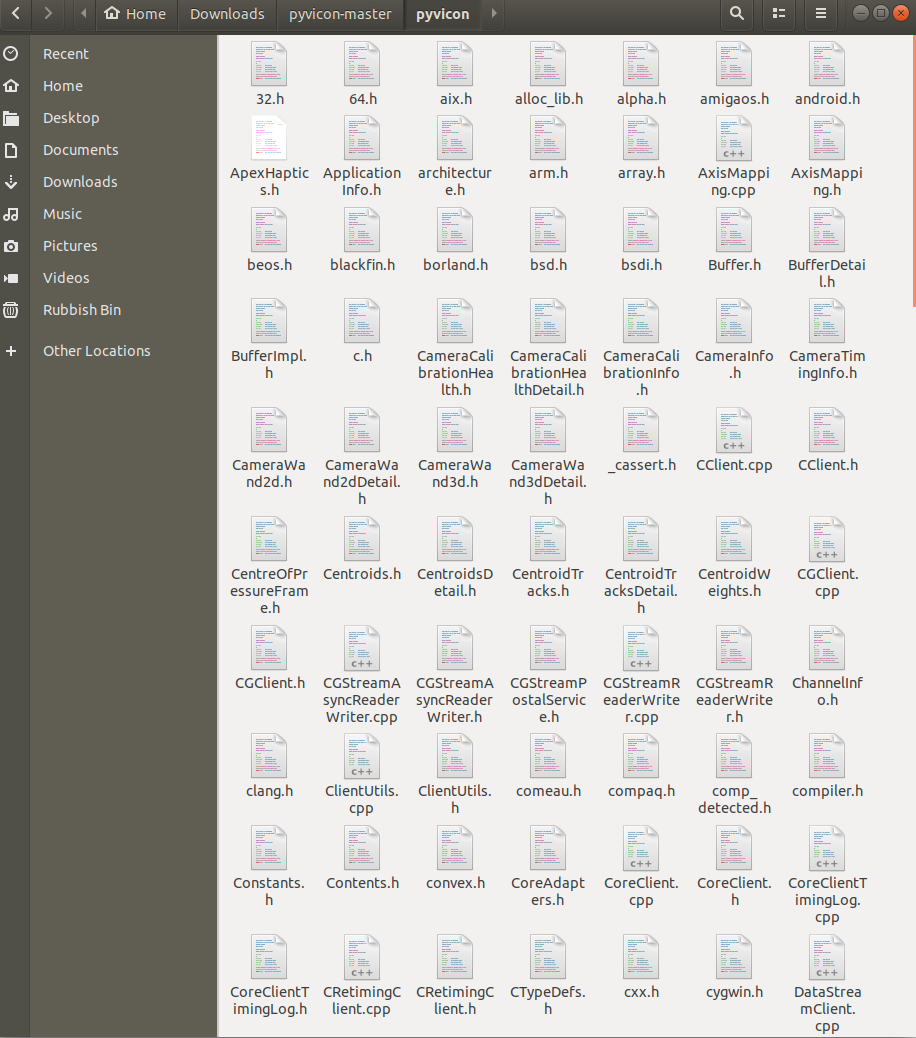
\includegraphics[width=1\linewidth]{Images/VirtualEnvironment/Four.png}
    \caption{.cpp and .h files of Vicon SDK merged into pyvicon folder}
    \label{fig:SDK17}
\end{figure}


% \begin{lstlisting}
% sudo find ~/Downloads/ViconDataStreamSDK_1.10.0.123216h -name "*.so" -exec cp {} /usr/local/lib/ \;
% \end{lstlisting}
% You also need to merge the .cpp and h files of Vicon SDK into pyvicon, run this 2 codes in the terminal that automates this, as seen in figure \ref{fig:SDK195}:
% \begin{lstlisting}
% sudo find ~/Downloads/ViconDataStreamSDK_1.10.0.123216h -name "*.cpp" -exec mv {} ~/Downloads/pyvicon-master/pyvicon/ \;
% \end{lstlisting}

% \begin{lstlisting}
% sudo find ~/Downloads/ViconDataStreamSDK_1.10.0.123216h -name "*.cpp" -exec mv {} ~/Downloads/pyvicon-master/pyvicon/ \;
% \end{lstlisting}
% \begin{figure}[H]
%     \centering
%     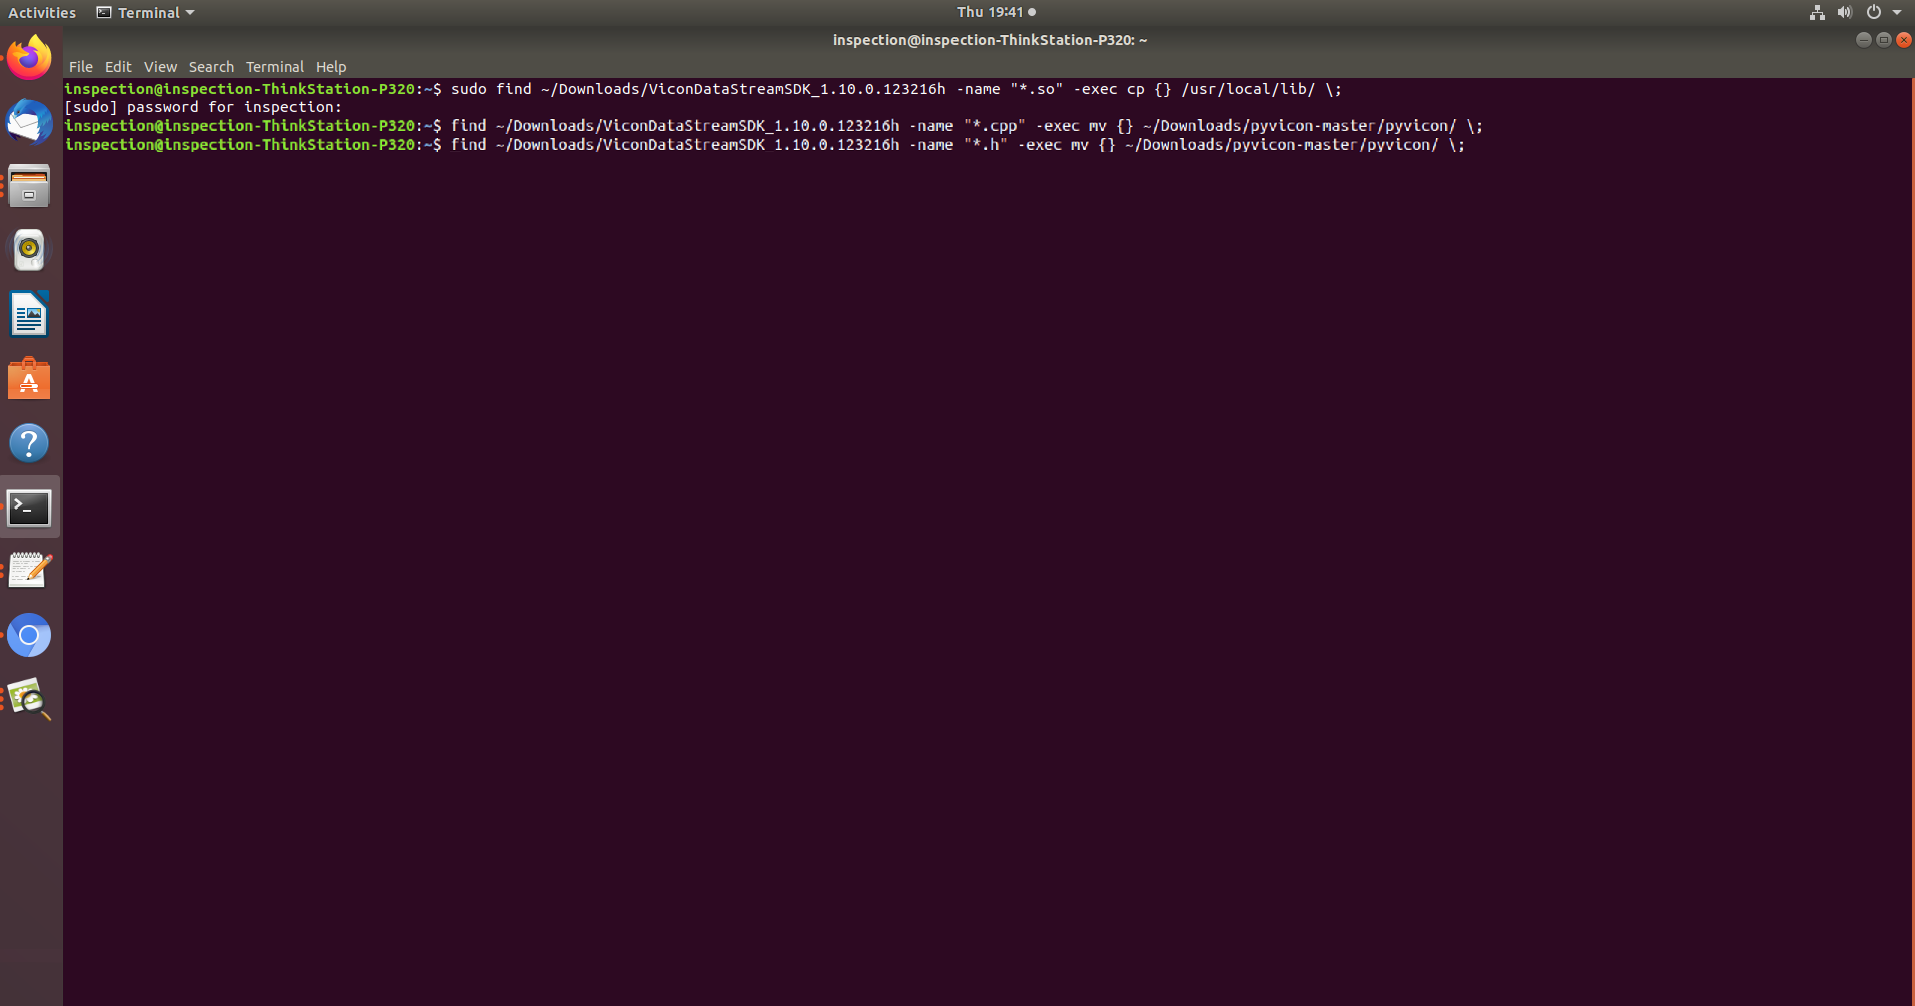
\includegraphics[width=1\linewidth]{Images/SDK195.png}
%     \caption{File merging codes}
%     \label{fig:SDK195}
% \end{figure}


\subsection{Installing Dependencies Packages}
A few dependencies are needed in order for pyvicon \& Mavproxy to work. Below are the dependencies and the corresponding versions that I used for a working setup: (Do note wxpython takes approximately 20 minutes to install, so be patient when you see the installation stall at wxpython, it is actually installing)

\begin{lstlisting}
    sudo apt-get install libgtk-3-dev 
    sudo apt remove modemmanager -y
    python3 -m pip install numpy==2.2.6
    python3 -m pip install  pathlib2==2.3.7.post1
    python3 -m pip install  matplotlib==3.10.9
    python3 -m pip install  opencv-python==4.13.0.92
    python3 -m pip install  Cython==3.2.4
    python3 -m pip install future==1.0.0
    python3 -m pip install  wxpython==4.2.5
\end{lstlisting}

Similarily, you can visit my Github page \href{https://matthewt0809.github.io/Vicon-Positioning-System-To-Pixhawk6C-Guide/}{https://matthewt0809.github.io/Vicon-Positioning-System-To-Pixhawk6C-Guide/} for the requirements.txt file that has all the dependencies listed in it, you can download this .txt file and install all dependencies by running the following code:
\begin{lstlisting}
    python3 -m pip install -r requirements.txt
\end{lstlisting}

\subsection{Setting up pyvicon}
To setup pyvicon wrapper, run the following code inside the \textit{Downloads/pyvicon-master} folder, as seen in figure \ref{fig:SDK18}:
\begin{lstlisting}
cd ~/Downloads/pyvicon-master
\end{lstlisting}
\begin{lstlisting}
python3 setup.py install
\end{lstlisting}
Test if the setup worked:
\begin{lstlisting}
    python3 -c "import pyvicon; print('OK')"
\end{lstlisting}
\begin{figure}[H]       
    \centering
    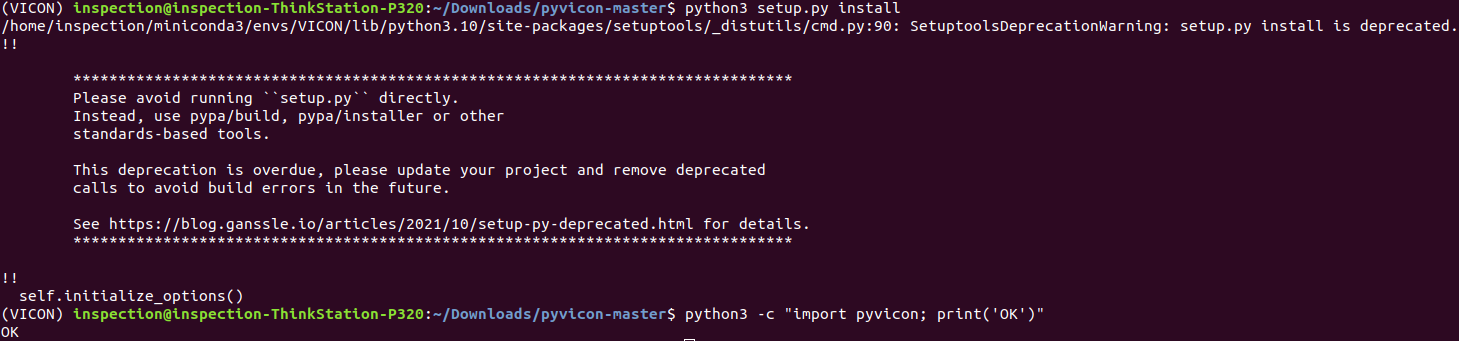
\includegraphics[width=1\linewidth]{Images/VirtualEnvironment/Seven.png}
    \caption{Overall setup of pyvicon}
    \label{fig:SDK18}
\end{figure}

If you see \textit{OK} printed in the terminal, you have successfully setup pyvicon. If there is an error, it is mostly arising from a mismatch in boost libraries. To keep the guide concise, please refer to appendix A for common debugging solutions that has worked for me. 


% You will also need to add \textit{$\sim$/.local/bin} to \textit{PATH} for pyvicon:
% \begin{lstlisting}
% echo 'export PATH="$HOME/.local/bin:$PATH"' >> ~/.bashrc && source ~/.bashrc
% \end{lstlisting}
% Both commands can be seen in figure \ref{fig:pyvicon4}
% \begin{figure}[H]
%     \centering
%     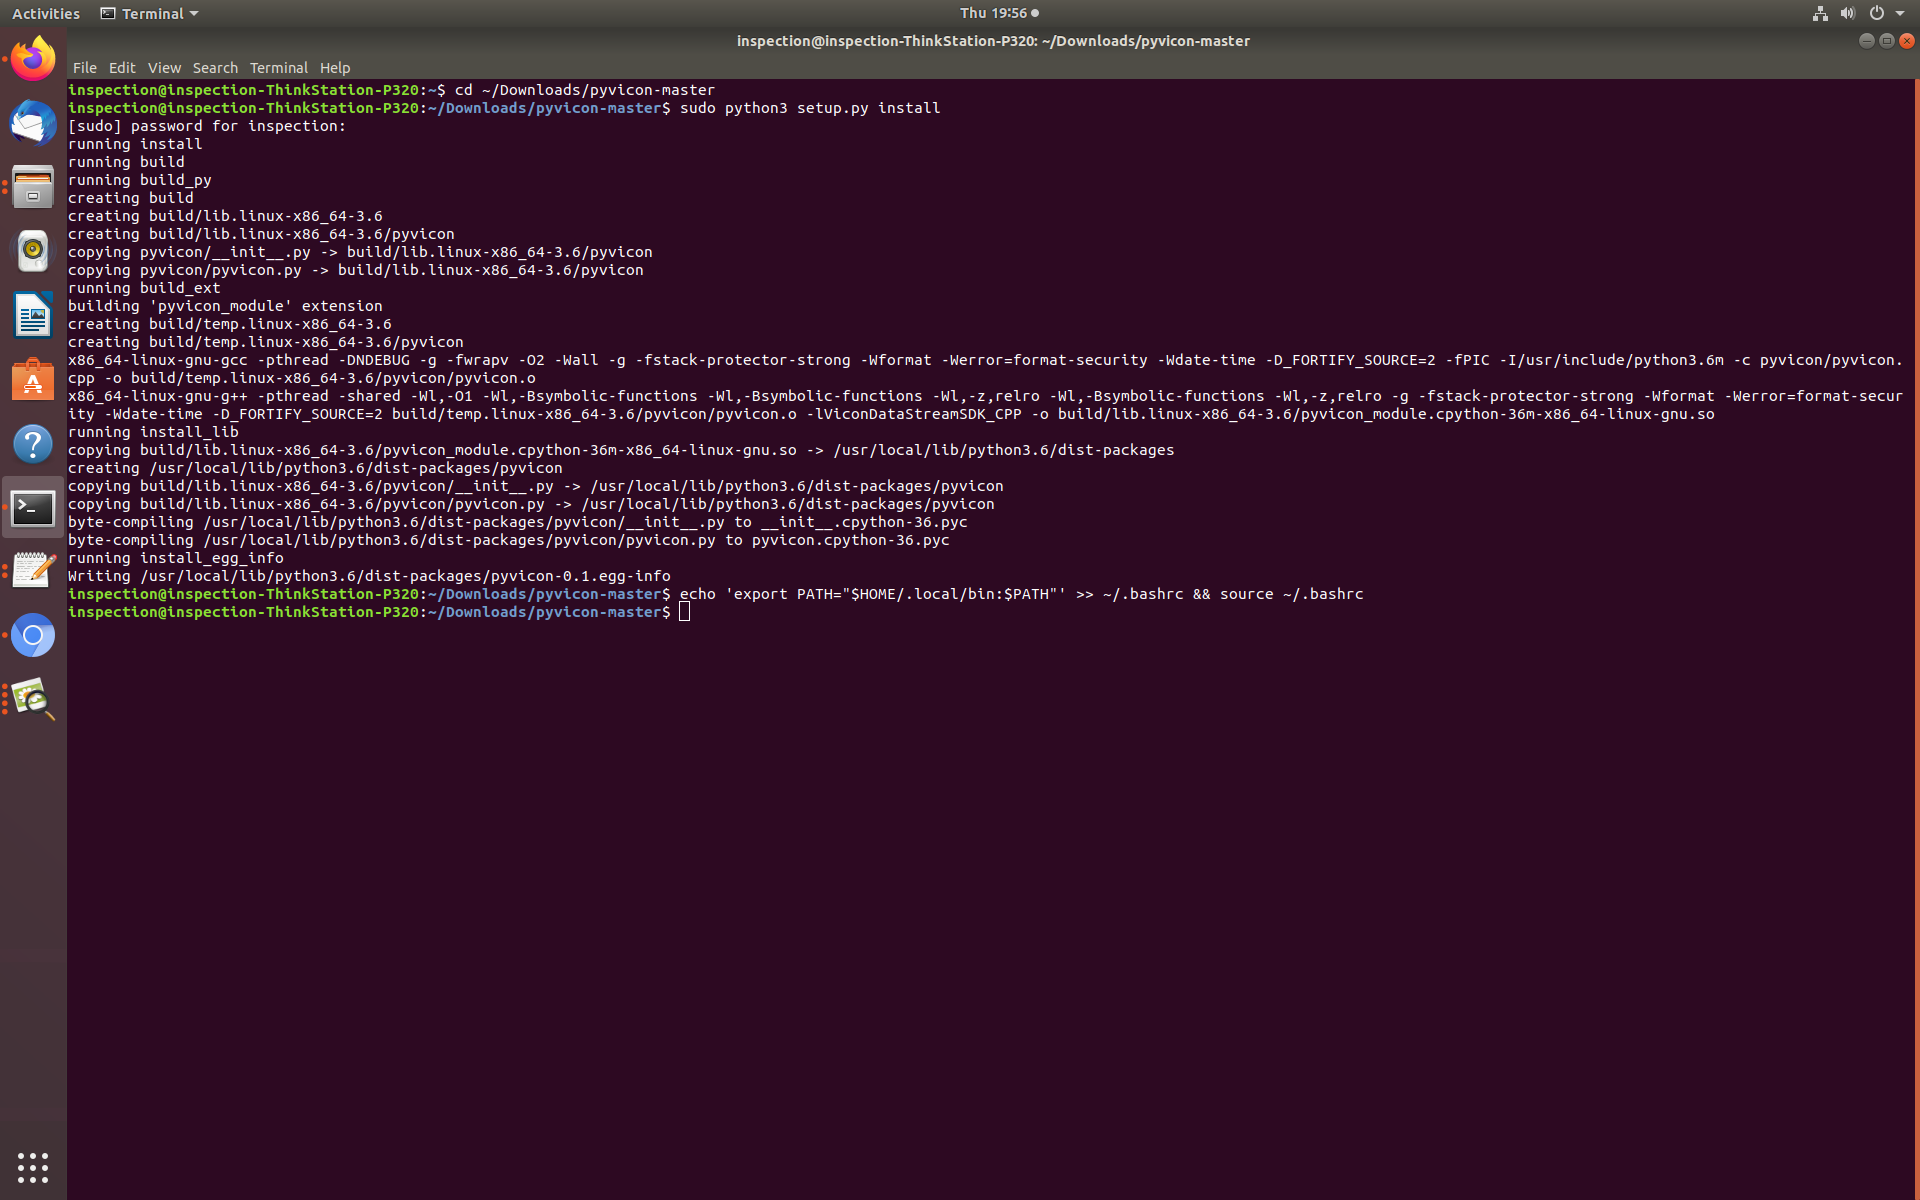
\includegraphics[width=1\linewidth]{Images/pyvicon4.png}
%     \caption{pyvicon setup and adding ~/local/bin to PATH}
%     \label{fig:pyvicon4}
% \end{figure}

% \begin{figure}[H]
%     \centering
%     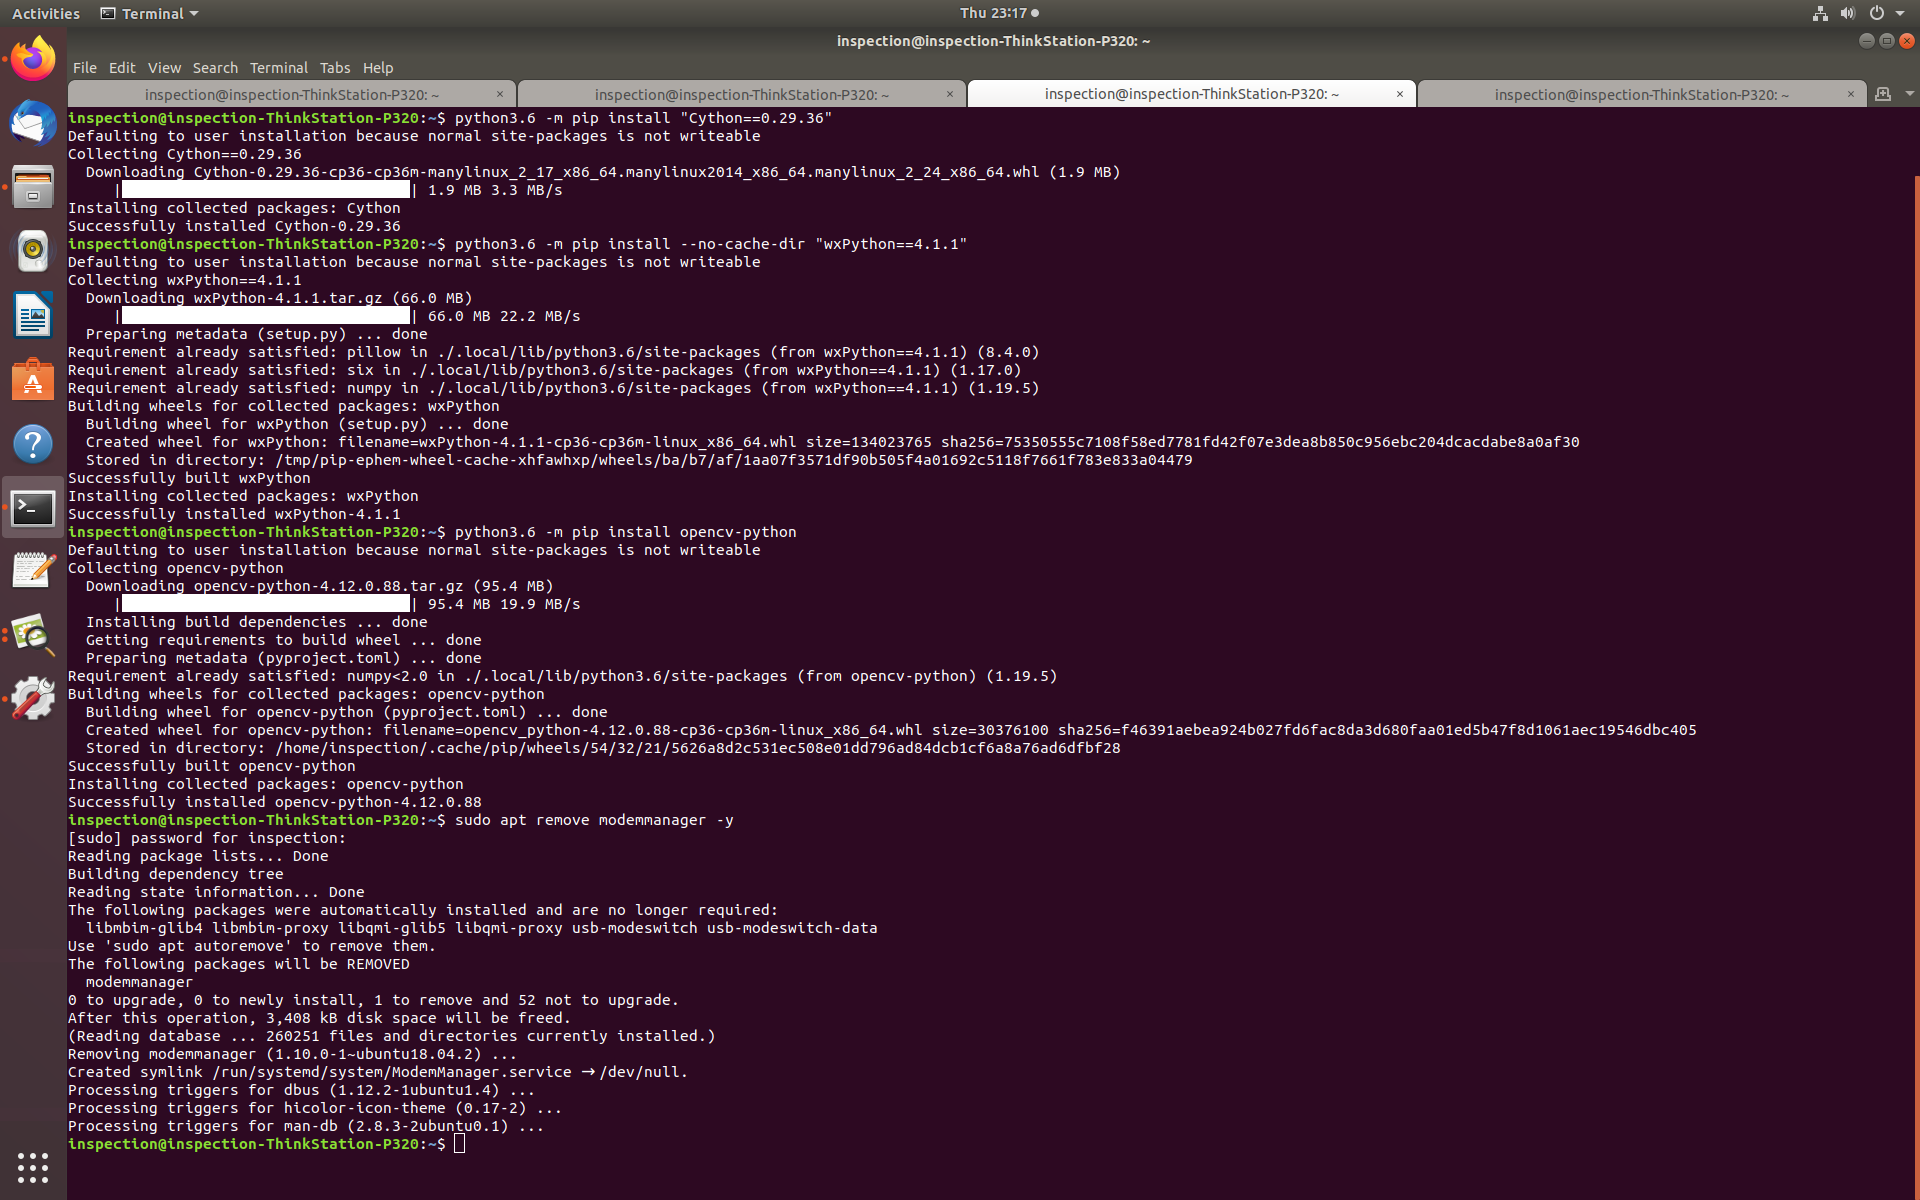
\includegraphics[width=1\linewidth]{Images/setup9.png}
%     \caption{Example of dependencies installation}
%     \label{fig:setup9}
% \end{figure}
\subsection{Installing Mavproxy \& Mavlink}
Next, the installation of Mavlink and Mavproxy. Run the following code as shown in figure \ref{fig:mavproxy11}: 
\begin{lstlisting}
    python3 -m pip install pymavlink==2.4.49
    python3 -m pip install mavproxy==1.8.74
\end{lstlisting}
\begin{figure}[H]
        \centering
        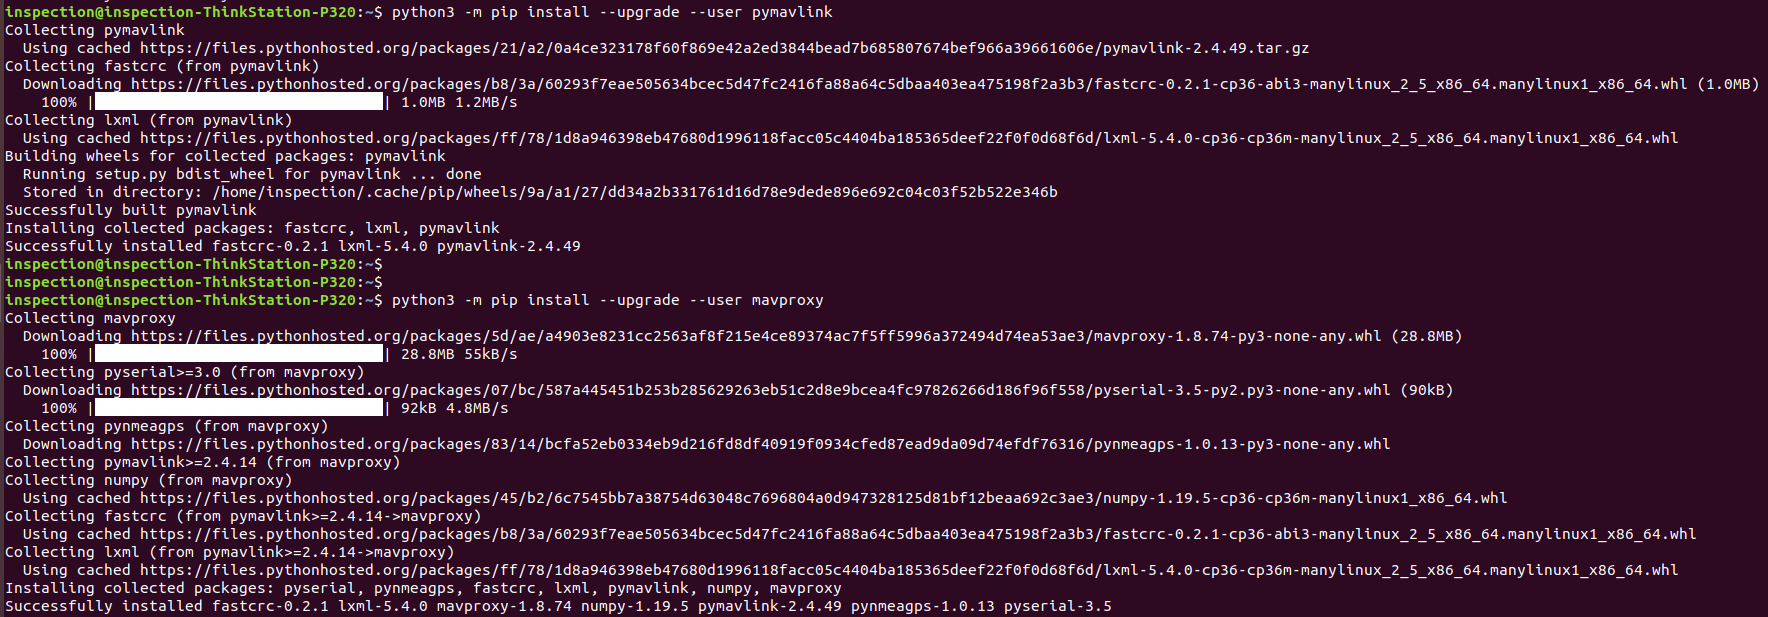
\includegraphics[width=1\linewidth]{Images/mavproxy11.png}
        \caption{Installing Mavproxy and Mavlink}
        \label{fig:mavproxy11}
\end{figure}

To test if your mavproxy installation is correct, run the following:

\begin{lstlisting}
    mavproxy.py --master :14550 --console --map
\end{lstlisting}

You should see the console and map window pops out as shown in figure \ref{fig:mavproxy2}. It will mention that link1 is down from the console, which is correct as you have not connected to your drone yet. 
\begin{figure}[H]
    \centering
    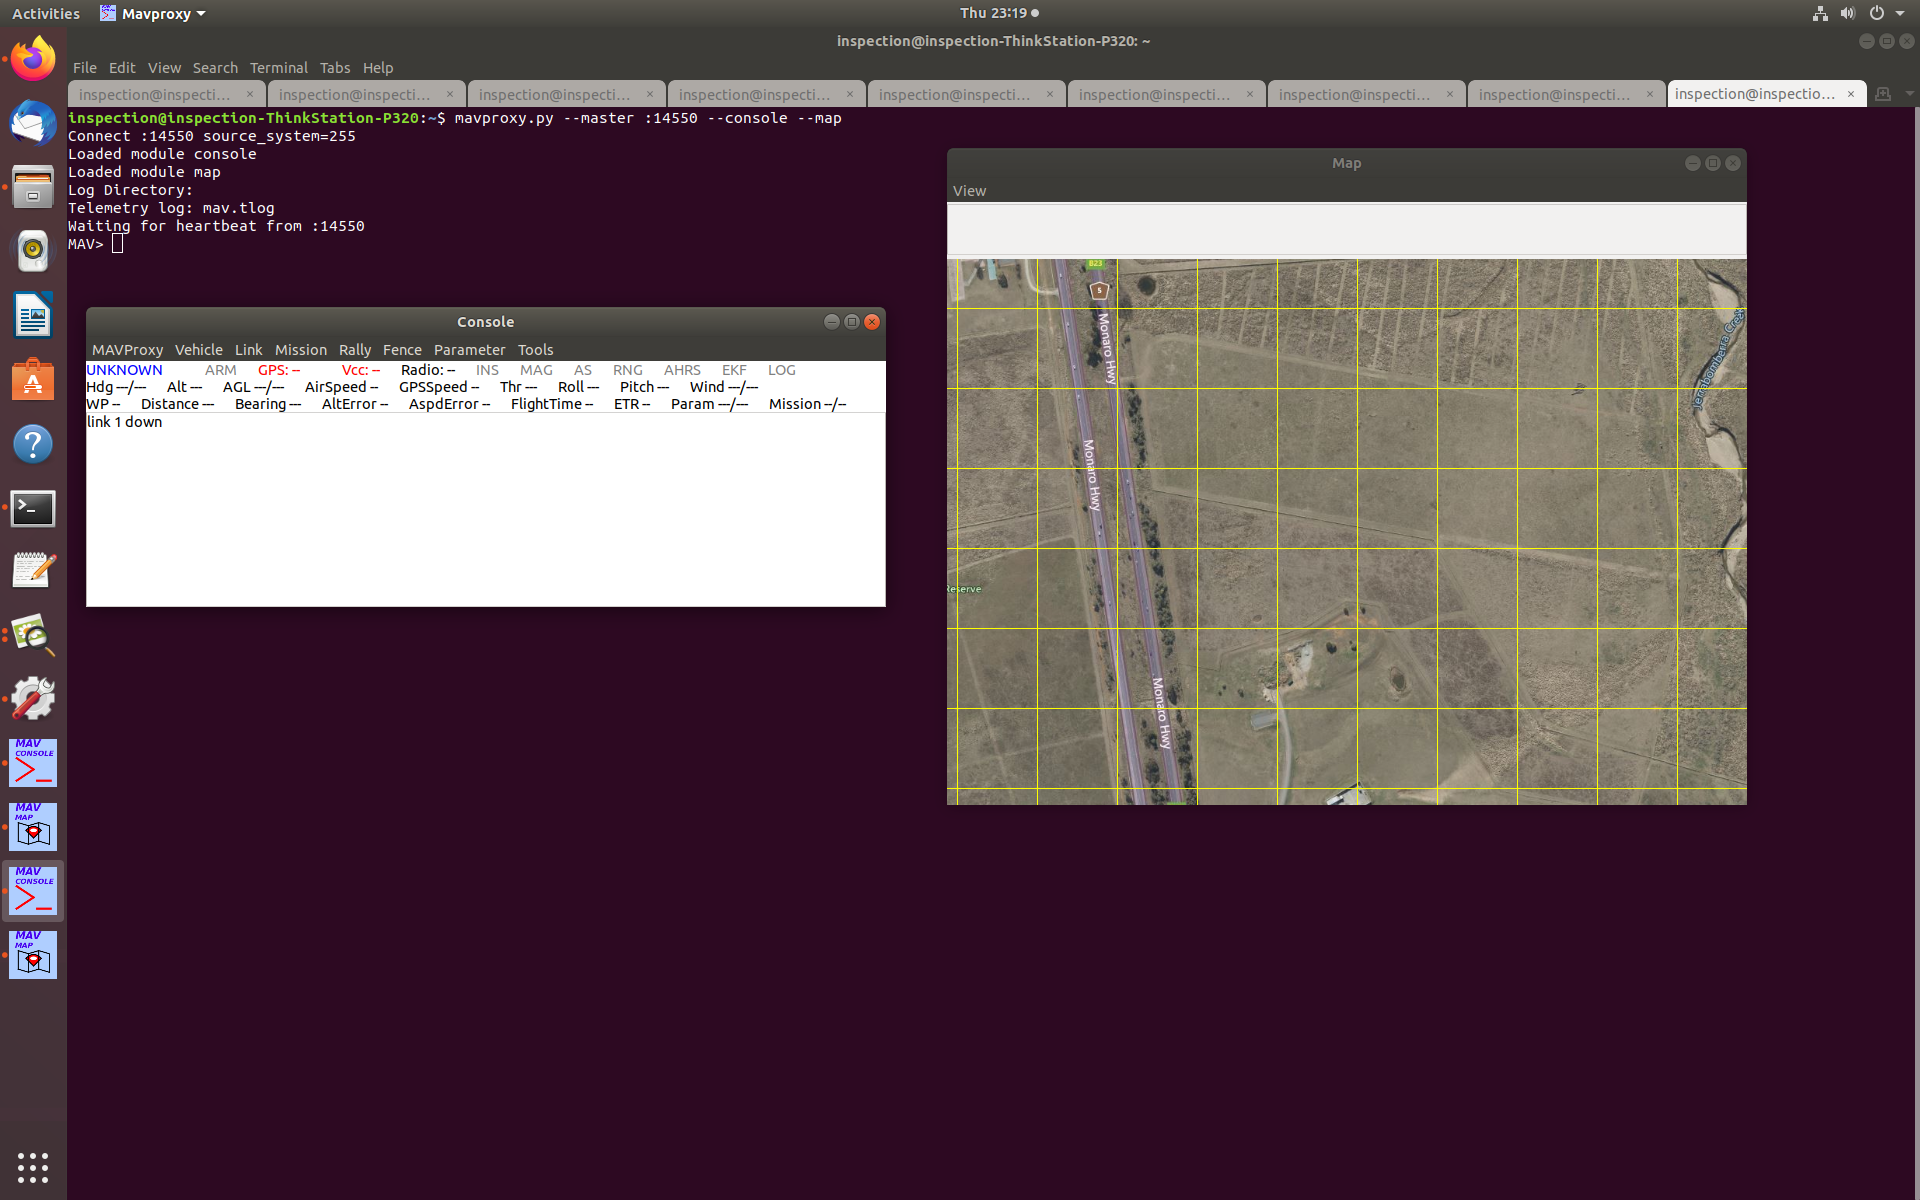
\includegraphics[width=1\linewidth]{Images/mavproxy2.png}
    \caption{Mavproxy console and map}
    \label{fig:mavproxy2}
\end{figure}

\subsection{Network setup}
Once all dependencies are installed, musculoskeletally move towards the Host PC with your GCS, locate the Vicon Ethernet Cable as shown in figure \ref{fig:hardware}. Connect the ethernet cable to your GCS. 
\begin{figure}[H]
    \centering
    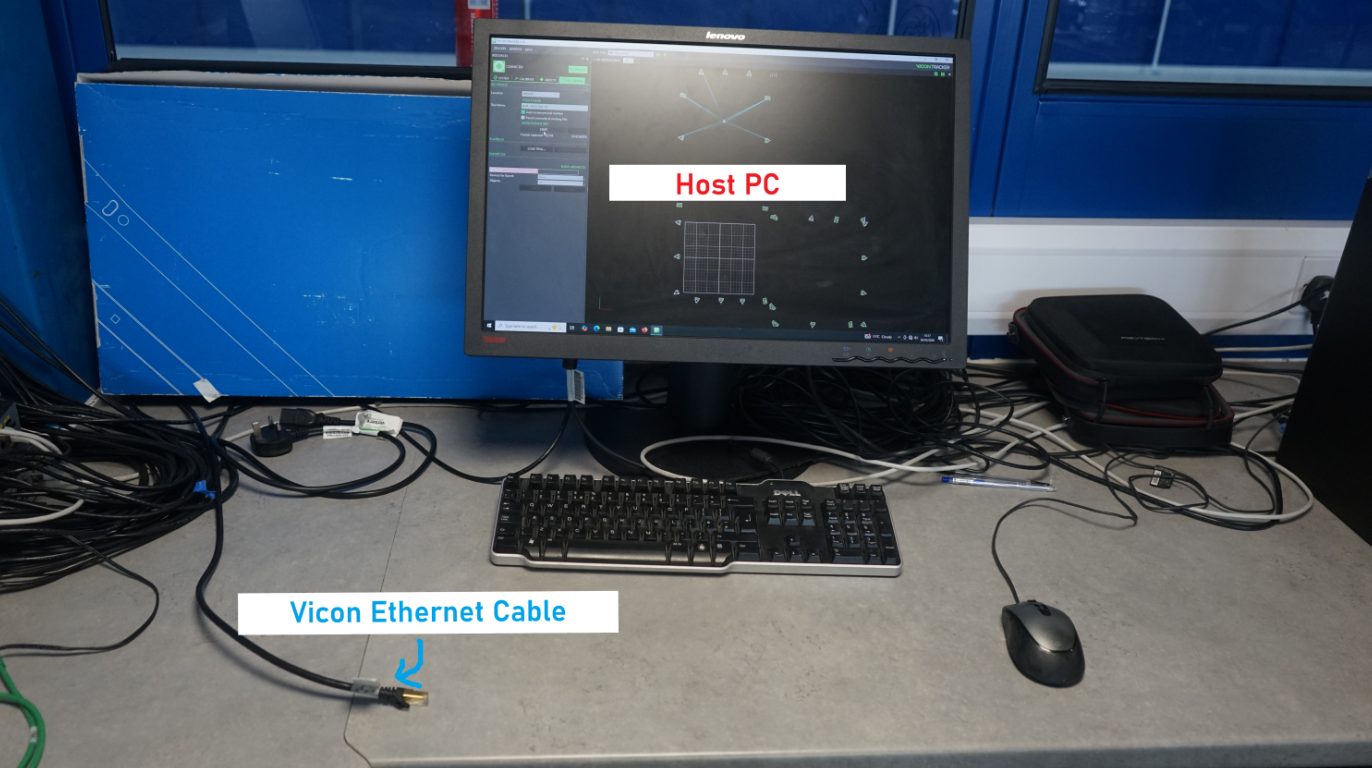
\includegraphics[width=1\linewidth]{Images/Hardware photo.png}
    \caption{Photo of Vicon Ethernet Cable}
    \label{fig:hardware}
\end{figure}

Once connected to the Ethernet cable, you will need to name your source of your Vicon positional data's ip address as \textit{vicon}, this can be done by typing this in Terminal, as shown in figure \ref{fig:network1}:\footnote{If you do some crawling around, you will note that this ethernet cable actually comes from within the flight arena, which would be useful if you want your GCS within the flight arena to test localisation later on.}

\begin{lstlisting}
    sudo nano /etc/hosts
\end{lstlisting}
\begin{figure}[H]
    \centering
    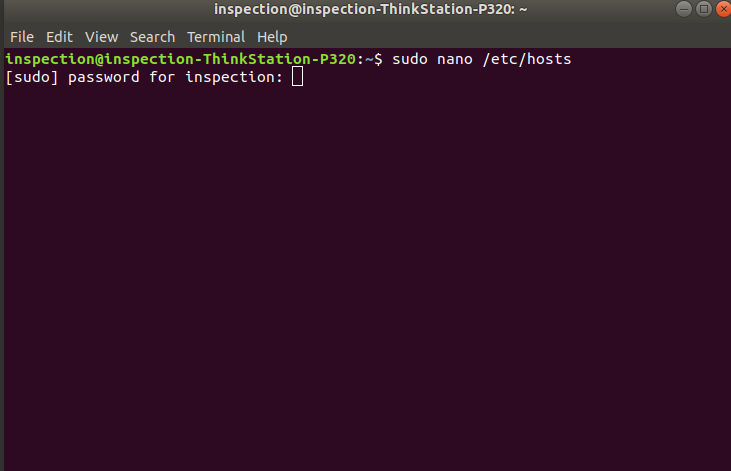
\includegraphics[width=0.8\linewidth]{Images/network1.png}
    \caption{Code for network name editing}
    \label{fig:network1}
\end{figure}

A window will show up like figure \ref{fig:network2}:

\begin{figure}[H]
    \centering
    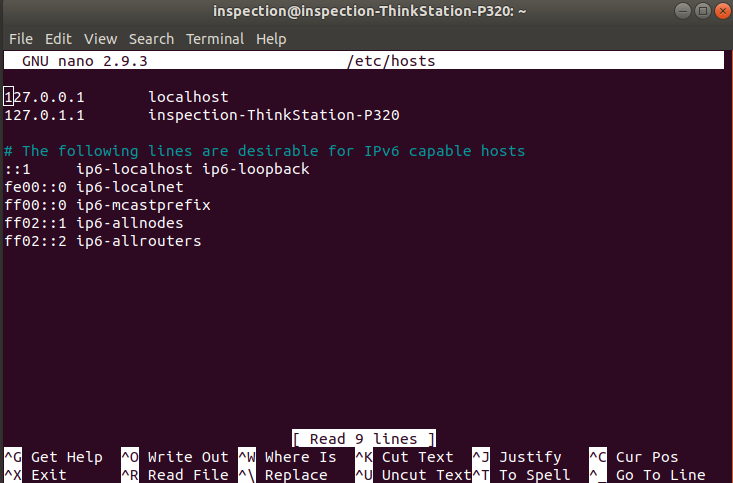
\includegraphics[width=0.8\linewidth]{Images/network2.png}
    \caption{Hosts file for network name editing}
    \label{fig:network2}
\end{figure}

Add \textit{192.168.0.218 vicon}\footnote{This IP address is empirical, if you use another router with a different network card, you will need to adjust the IP address accordingly.} as shown in figure \ref{fig:network3}. Then press Ctrl+O to save the changes, Ctrl+X to exit the window. 
\begin{figure}[H]
    \centering
    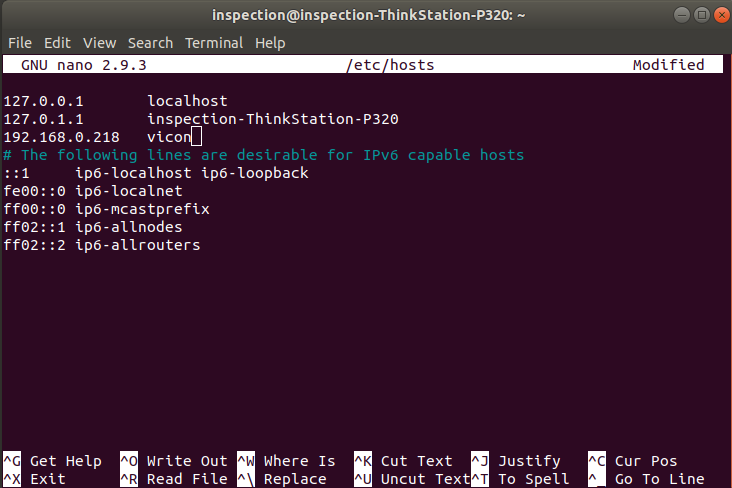
\includegraphics[width=0.8\linewidth]{Images/network3.png}
    \caption{Adding vicon IP address to hosts file}
    \label{fig:network3}
\end{figure}
Test your connection to vicon via ethernet cable by doing: 
\begin{lstlisting}
    ping vicon
\end{lstlisting}

If \textit{64 bytes from vicon (192.168.0.218): icmp\_seq=1 ttl=128 time=0.517ms} messages begin appearing like shown in figure \ref{fig:network5}, you have a correct connection between Vicon Tracker and your computer!
\begin{figure}[H]
    \centering
    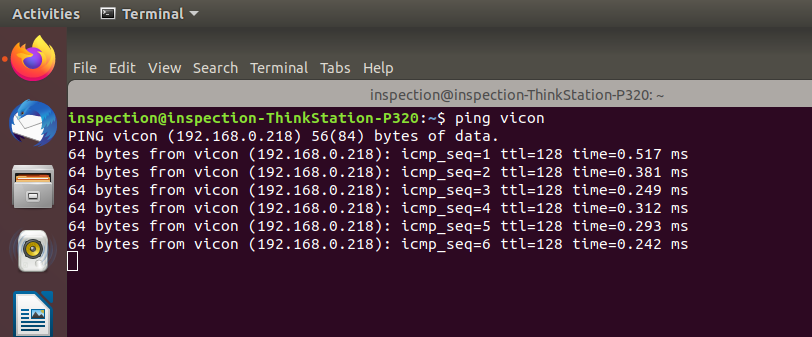
\includegraphics[width=0.8\linewidth]{Images/network5.png}
    \caption{Successful ping to vicon}
    \label{fig:network5}
\end{figure}
